% Created 2020-12-01 Tue 15:09
% Intended LaTeX compiler: pdflatex
\documentclass[number,5p]{elsarticle}

\usepackage[utf8]{inputenc}
\usepackage[T1]{fontenc}
\usepackage{graphicx}
\usepackage{grffile}
\usepackage{longtable}
\usepackage{wrapfig}
\usepackage{rotating}
\usepackage[normalem]{ulem}
\usepackage{amsmath}
\usepackage{textcomp}
\usepackage{amssymb}
\usepackage{capt-of}
\usepackage{hyperref}
\usepackage{wasysym}
\usepackage{gensymb}
% \usepackage{physics}
\usepackage{hepnames}
\usepackage[inline]{enumitem}

% standadized SI units
\usepackage[per-mode=symbol, range-units=single, binary-units=true]{siunitx}
\DeclareSIUnit\clight{\text{\ensuremath{c}}} % redefine light speed symbol
\DeclareSIUnit\momentum{\GeV\per\clight} % momentum in GeV/c
\DeclareSIUnit\tmom{(\momentum)^2} % 4-momentum squared
\DeclareSIUnit\atom{\text{atoms}} 
\DeclareSIUnit\event{\text{events}} 
\DeclareSIUnit\KB{\text{KB}} 

% tables with separate column and row label
\usepackage{booktabs}
\newcommand\headercell[1]{%
\smash[b]{\begin{tabular}[t]{@{}c@{}} #1 \end{tabular}}}

% for unbreakable paragraphs
\usepackage{ragged2e}

\begin{document}

\begin{frontmatter}	
  \title{The KOALA Experiment for (anti)proton-proton Elastic Scattering}
  \date{\today}

  \author[ikp]{Yong Zhou\corref{cor}}
  \ead{y.zhou@fz-juelich.de}
  \author[ikp]{Huagen Xu}

  \author[ikp]{Ulf Bechstedt}
  \author[ikp]{Jürgen Böker}
  \author[ikp]{Nils Demary}
  \author[ikp]{Frank Goldenbaum}
  \author[ikp]{Dieter Grzonka}
  \author[ikp]{Jan Hetzel}
  \author[muenster]{Alfons Khoukaz}
  \author[ikp]{Franz Klehr}
  \author[ikp]{Thomas Krings}
  \author[muenster]{Lukas Lessmann}
  \author[muenster]{Christian Mannweiler}
  \author[ikp]{Dieter Prasuhn}
  \author[ikp]{Steffen Quilitzsch}
  \author[gsi,bochum,ikp]{James Ritman}
  \author[ikp]{Susan Schadmand}
  \author[ikp]{Thomas Sefzick}
  \author[ikp]{Rolf Stassen}
  \author[zea]{Peter Wüstner}

  \cortext[cor]{Corresponding author}
  % \fntext[fn1]{Present address: Institute of Modern Physics, Chinese Academy of Sciences, Lanzhou, 730000, China}
  % \fntext[fn2]{Present address: GSI Helmholtzzentrum für Schwerionenforschung GmbH, Darmstadt, 64291, Germany}

  \address[ikp]{Institut für Kernphysik, Forschungszentrum Jülich, Jülich, 52425, Germany}
  \address[muenster]{Institut für Kernphysik, Universität Münster, Münster, 48149, Germany}
  \address[bochum]{Ruhr-Universität Bochum, Bochum, 44780, Germany}
  \address[gsi]{GSI Helmholtzzentrum für Schwerionenforschung GmbH, Darmstadt, 64291, Germany}
  \address[zea]{Zentralinstitut für Engineering, Elektronik und Analytik, Forschungszentrum Jülich, Jülich, 52425, Germany}


  \begin{abstract}
    % Cross section data of (anti)proton-proton elastic scattering is important
    % for the study of nuclear forces and also provides necessary ingredients in
    % the modeling of meson production and other nuclear reactions at intermediate energies.

    % A good understanding of the nucleon-nucleon interaction is one of the principal
    % goals of nuclear and hardon physics.
    % The KOALA experiment is initially proposed to measure the antiproton-proton elastic scattering at HESR, which the data are crucial input for the absolute luminosity determination of PANDA experiment.
    The KOALA experiment measures the differential cross section
    of (anti)proton-proton elastic scattering over a wide range of four-momentum
    transfer squared $0.0008 < |t| < \SI{0.1}{\tmom}$.
    These data are essential input for the luminosity detector of the PANDA experiment to reach the desired absolute precision.
    % The forward scattering parameters and the absolute luminosity can be deduced
    % by analyzing the characteristic shape of the differential cross section spectrum.
    The experiment is based on fixed target kinematics and uses an internal hydrogen cluster jet target.
    The wide range of $|t|$ is achieved by measuring the total kinetic energy of the recoil
    protons near \SI{90}{\degree}.
    The recoil detector consists of silicon and germanium single-sided strip sensors.
    The energy resolution of the recoil detector is approximately \SI{30}{\keV} (FWHM).
    %and the angular resolution better than \SI{0.1}{\degree}.
    A forward detector consisting of two layers of plastic scintillators measures the
    elastically scattered beam particles in the forward direction close to the beam
    axis.
    By requiring a coincidence of the forward detector with the recoil detector, the large background at small recoil angles is suppressed, thereby improving the identification of elastic scattering events in the low $|t|$ range.
    The KOALA setup has been installed and commissioned with proton beam at COSY in order to validate the detector by measuring the proton-proton elastic scattering.
    % The full system of KOALA is described in this article and test beam results
    % verifying the design and the performance are presented.
    The results from this commissioning are presented here.
    % The experiment ran smoothly and the preliminary results verify that the designed range of |t| could be achieved with the help of
    % the forward detector.

  \end{abstract}

  \begin{keyword}
    proton-proton elastic scattering 
    \sep solid-state detector
    \sep PMT
    \sep TOF-E
    \sep plastic scintillator
    \sep four momentum transfer squared
  \end{keyword}

%  \newpageafter{abstract}
\end{frontmatter}


% \newpage
% \tableofcontents
% \newpage

\section{Introduction}
\label{sec:introduction}

\begin{figure*}[htbp]
	\centering
	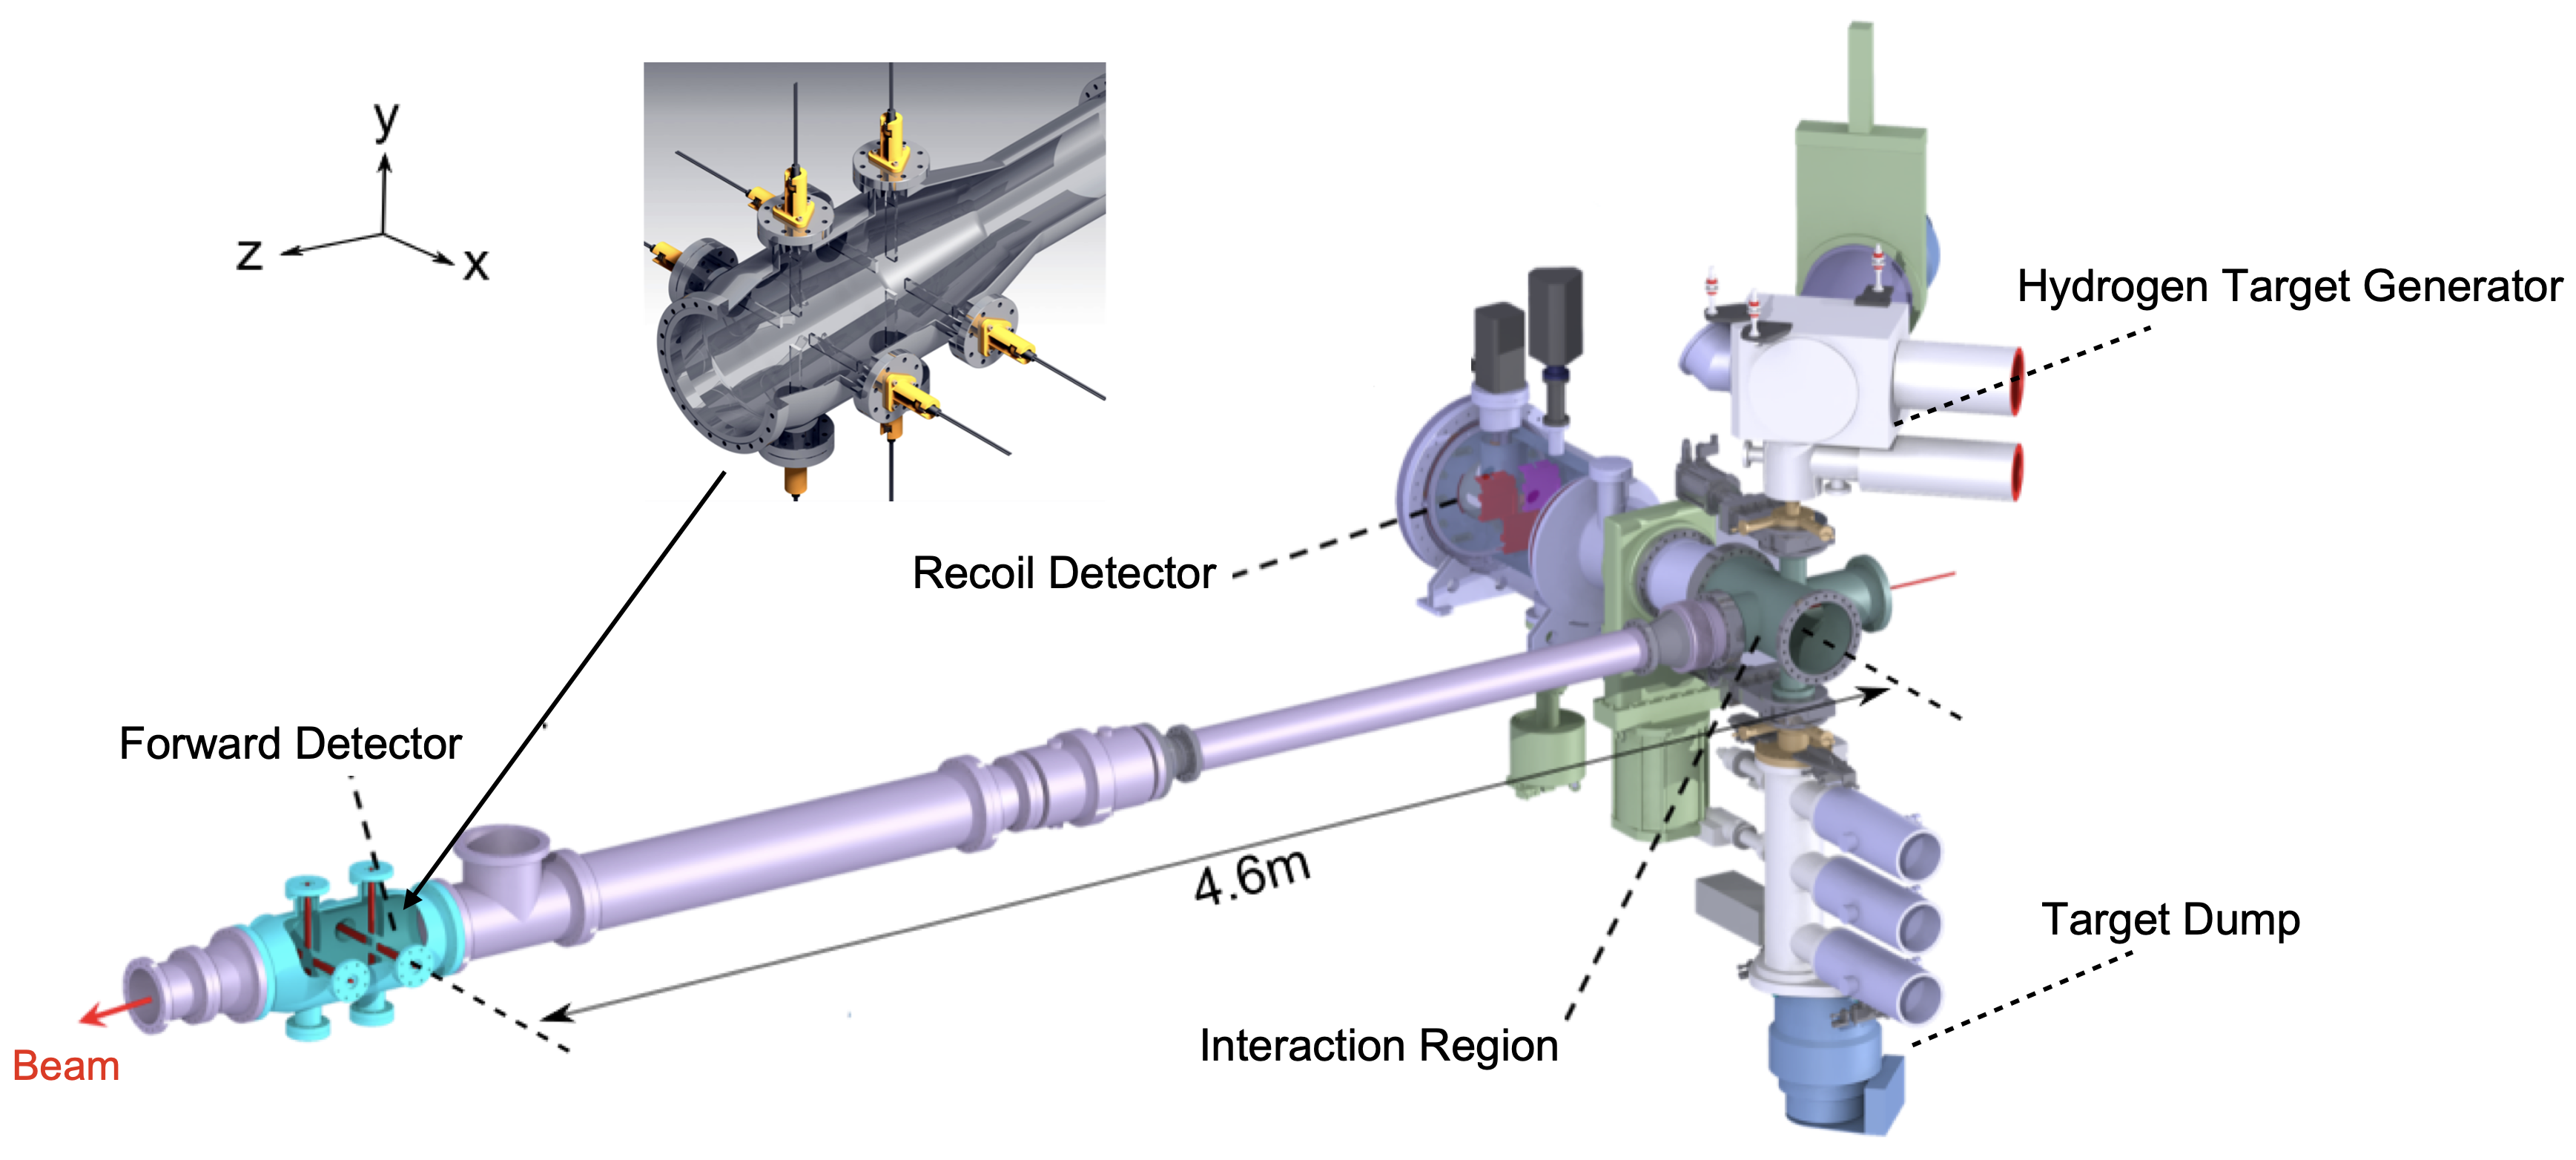
\includegraphics[width=0.8\textwidth]{./koala_setup_new.png}
	\caption{3D visualization of the KOALA setup at COSY. An expanded view of the
  forward detector is shown in the inset, in which the aluminium tubes are not shown.}
	\label{fig:setup}
\end{figure*}

The KOALA experiment (\textbf{K}ey experiment f\textbf{O}r P\textbf{A}NDA \textbf{L}uminosity determin\textbf{A}tion) is a fixed-target experiment that measures the differential cross-section of $\bar{p}p$ or $pp$ elastic scattering over $0.0008 < |t| < \SI{0.1}{\tmom}$.
It will measure $\bar{p}p$ elastic scattering at the future HESR ring of FAIR \cite{FAIR} in the beam momentum range from
\SIrange{1.5}{15}{\momentum} and a summary of its physics program can be found
in \cite{panda}.
The cross-section data obtained from the KOALA experiment is an essential input for the PANDA luminosity detector to
reach an absolute precision of ${\Delta L}/{L} < \SI{5}{\percent}$ \cite{lmd_tdr}.
Before the intallation at HESR, the KOALA experiment is first commissioned with
proton beam from COSY \cite{COSY} in the beam momentum range from
\SIrange{1.5}{3.4}{\momentum}.

The KOALA experiment covers the kinematic regions where the
Coulomb interaction, the CNI and the nuclear interaction have different relative importance.
The so-called Coulomb normalization method \cite{bernard1987real,jenni2008atlas}
can be used within the Coulomb dominated kinematic region.
This enables the possibility to determine \({\sigma}_{tot}\), \(b\), \(\rho\) as well as
the absolute luminosity by analyzing the characteristic shape of the $dN/dt$
spectrum (i.e. relative differential cross section) \cite{koala_article}.
The absolute differential cross section can be normalized by the data in the
Coulomb region.

Due to limitations from the beam pipe aperture and the beam emittance,
it is extremely difficult to measure the forward emitted elastically scattered particle over a wide range of scattering angles.
The recoil measurement technique, \textit{i.e.}, the precise measurement of both the recoil angle and the kinetic energy of the recoil proton, 
is used to determine the differential elastic scattering cross section in the
KOALA experiment.
Identification of the elastic scattering events is based on the correlation between the recoil angle and the kinetic energy.
A recoil detector based on this idea has already been built and the method of
recoil measurement technique was verified using proton beam
\cite{koala_article,recoil_article}.
However, it was found in these tests that the identification of elastic events at small recoil angles was limited by the low-energy background events.
%which correspond to $|t| < \SI{0.002}{\tmom}$.

% To reach the remaining range \(0.0008 < |t| < 0.001\) \((GeV/c)^2\) in KOALA, a coincidence measurement between the recoil proton and scattering beam particle is proposed to suppress the background contamination.
% A time-sensing forward detector with a limited coverage range at small scattering angle is designed and built for this purpose. 
% the coincidence measurement between the recoil proton and scattering beam particle is proposed.
Background at low kinetic energy is mainly from inelastic scattering processes.
In order to sufficiently suppress the background across the desired $|t|$ range,
a forward hodoscope based on fast-timing plastic scintillator is employed
to measure the elastically scattered beam particle in coincidence with the kinematic partner in the recoil detector.
This full setup of the KOALA experiment consisting of the recoil detector, the newly-built
forward detector, the cluster jet target and other upgraded components was installed at COSY.
Several tests using proton beams have been carried out to verify the design and the performance.
In the following sections,  the full system of the KOALA experiment is described and the preliminary results from the beam commissioning are presented.

\section{Experimental setup at COSY}
\label{sec:setup}

The KOALA setup is installed at a straight section in the COSY storage ring.
It consists of three arms as shown in Fig. \ref{fig:setup}: the hydrogen
cluster jet target arm, the recoil arm and the forward arm.
All components in these arms are installed in the same vacuum volume as the
proton beam.

The hydrogen cluster jet target arm connects the scattering chamber vertically (Y-axis) with the target generator above and the target beam dump below.
The recoil arm is oriented along the X-axis.
The chamber holding the recoil detector is separated from the scattering chamber by a vacuum gate valve.
This valve is used for staged pumping of the recoil chamber during the
preparation of the experiment and separates the detector and the beam vacuum when
either is not within the nominal pressure range for operation.
The forward chamber is located about \SI{4.6}{\meter} downstream from the
central axis of the cluster target jet.
It is connected to the scattering chamber by two beam pipes with diameters of \SI{90}{\mm} and \SI{200}{\mm}.
\subsection{Hydrogen cluster jet target}
\label{sec:target}

A thin hydrogen target, which can be operated under ultra-high vacuum
conditions, is critical for the success of the KOALA experiment.
First off, the energy loss of recoil protons should be minimal before impinging
on the recoil sensor so that an accurate determination of its kinetic energy is possible.
Second, the target thickness along the COSY beam axis determines
the spread of the vertex distribution of the beam-target interaction.
Since there is no tracking device in the KOALA setup, this spread will deteriorate the
angular resolution as well as the shape of the energy spectrum.

The cluster jet is a type of target structure commonly used in internal target experiments, that require moderate
target densities with the lowest material budget.
The hydrogen cluster jet is generated by pressing the hydrogen gas at high
pressures (about \SI{18}{\bar}) and low temperatures (\SIrange{20}{30}{\K})
through a Laval nozzle \cite{cluster_target}. 
The hydrogen cluster jet target in the KOALA setup was used previously in the ANKE experiment
\cite{cluster_target_new}.
The target has been upgraded with a new collimator, so that a smaller target thickness is achieved.
The cluster jet profile was measured by using a probing rod when no accelerator beam was circulating inside COSY.
A typical thickness of \SI{1.5}{\mm} (FWHM) at the interaction point (IP) was determined.
The areal density is estimated to be \SI{e14}{\atom\per\cm\squared}.
% The full width at half maximum (FWHM) of the cluster jet beam is measured
% It is $\sim\SI{1.5}{\mm}$ thick close to the interaction point (IP).
Typically, COSY stores $10^{10}$ protons and the beam has a revolution frequency
of about \SI[per-mode=power]{e6}{\per\second}, thus giving an estimated luminosity of $L \approx 10^{30}\si{cm^{-2}s^{-1}}$.
% The typical proton beam intensity of COSY is about
% \SI{e16}{\atom\per\second},
% for the KOALA experiment at COSY.

\subsection{Recoil detector}
\label{sec:recoil}

The recoil detector records the proton from the
elastic scattering and measures its total kinetic energy and recoil angle.
For elastic scattering of two particles with the same mass,
the kinetic energy of the recoil proton \(T_p\) is proportional to $|t|$ with \(|t| = 2m_pT_p\), where \(m_p\) is the proton mass.
For $|t|_{max}=\SI{0.1}{\tmom}$, \(T_p \approx \SI{54}{\MeV}\).
The recoil detector is required to measure deposited energies of up to \SI{60}{\MeV}.
The angular resolution of the recoil detector is required to be better than \SI{0.1}{\degree}.
% The lower range is determined to have an effective suppression of the noise of the
% readout electronics.
Position-sensitive solid-state sensors are ideal material to achieve these
requirements and suitable to be used in ultra-high vacuum environment (\SI{e-8}{\milli\bar}).
Due to the strong variation of the recoil particle's kinetic energy with the angle,
the optimal thickness of the sensor thickness varies strongly with the recoil angle.
Since commercially-avalibale silicon sensors are not thick enough to measure the deposited energies up to \SI{60}{\MeV},
thick germanium sensors were developed and manufactured at IKP to cover the larger $|t|$ region.

\begin{figure}[htbp]
  \centering
  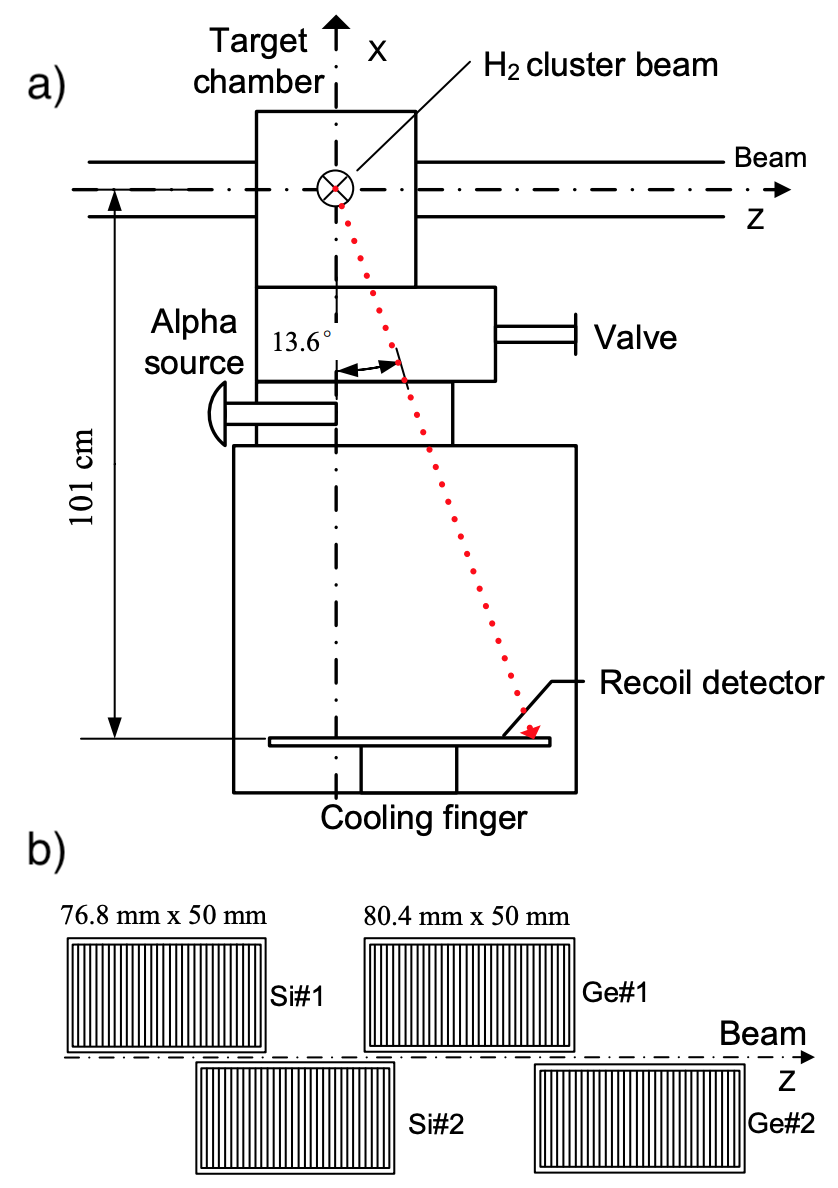
\includegraphics[width=0.35\textwidth]{./recoil_schematic.png}
  \caption{(a) Schematic view of the recoil detector configuration, seen from the
    top; (b) Layout of the four recoil sensors, seen from the interaction point.}
  \label{fig:recoil_schematic}
\end{figure}
% A mixed layout of the recoil detector setup is adopted as shown in Fig. \ref{fig:recoil_schematic}.
The recoil detecotr consists of two single-sided silicon strip sensors of same
thickness (\SI{1}{\mm}) at small recoil angles, where the maximal recoil energy
is \SI{12}{\MeV}. Two single-sided germanium strip sensors of different
thickness (\SI{5}{\mm} and \SI{11}{\mm}) are used at larger recoil angles, where
the recoil angle varies from \SIrange{12}{54}{\MeV}.
The sensors are arranged along the COSY beam axis with staggered placement in the Y-axis.
% The thickness of each sensor is optimized for the energy range it measures: \SI{1}{\mm} for Si1
% and Si2, \SI{5}{\mm} for Ge1 and \SI{11}{\mm} for Ge2.
The detector plane is installed \SI{90.4}{\cm} from the beam-target center
and covers a range of recoil angle $\alpha$ ($=\SI{90}{\degree}-\theta$) from \SIrange[range-units=repeat]{-1.8}{15}{\degree}.
The silicon sensors have a sensitive area of $76.8 \times \SI{50}{\mm\squared}$, which is
segmented into 64 strips of \SI{1.2}{\mm} pitch.
The germanium sensors have a sensitive area of \(80.4 \times \SI{50}{\mm\squared}\), which is segmented into 67 strips of \SI{1.2}{\mm} pitch.
% This gives an angular resolution of about \SI{0.08}{\degree}.
By design, neighboring sensors have an overlapping region, which is symmetric
relative to the COSY beam axis (Si1 and Si2 have 20 overlapping strips, Si2 and Ge1
have 9 overlapping strips, Ge1 and Ge2 have 10 overlapping strips).
The overlapping strips are used to correct systematic errors such as a beam position asymmetry.

The recoil sensors are read out by a combination of charge-sensitive preamplifiers (MPR16 for the strips, MPR1 for the rear side) and timing filter amplifiers (MSCF16), from Mesytec \cite{mesytec}. 
MSCF16 integrates a shaping amplifier and a leading edge discriminator in the
same module and outputs an amplitude signal and a timing signal, which are used
for the energy and time measurement, respectively.
% Strips at larger recoil angles are read out by a single channel without sacrificing the angular resolution.
Since only 180 readout channels are available, the readout for some of the
strips has been combined, thus there are in effect 48 channels on Si1, 64
channels on Si2, 32 channels each on Ge1 and Ge2, and 4 channels for the rear sides
of the four sensors. 

The germanium sensors need to be operated at low temperature.
Thus, an active cooling system was implemented for the recoil detector.
% Soild-state sensors (especially germanium) need a low and stable operating
% temperature to optimize the energy resolution.
The temperature of the recoil sensors is monitored by four temperature sensors attached to the detector holder.
The operating temperature can be actively adjusted by a combination of a pulse
tube cold head \cite{pt30} and two heating resistors, which are affixed and thermally coupled to the detector cold plate.
A study of the performance of the recoil sensors in the laboratory using
$^{244}Cm$ as $\alpha$ source \cite{recoil_article} showed that the working temperature with the best energy resolution is
\SI{125}{\kelvin}.

The $\alpha$ source for the energy calibration (Sec. \ref{sec:energy_calibration}) is also installed inside the recoil chamber and fixed on a linear motion feedthrough rod.
During the experiment, the rod is in a parking position that is hidden from the
recoil detector by the scattering chamber;
when calibration is needed, the rod is pushed to the chamber center and the sources face the recoil sensors directly.
Thus, the recoil detector can be calibrated regularly when no beam is in the storage ring.

More technical information and the detailed performance tests of the recoil detector can be found in \cite{recoil_article}.

\subsection{Forward detector}
\label{sec:fwd}

The forward detector measures the arrival time of the elastically scattered beam proton in the
forward direction.
The arrival time is used as the start time to calculate the time-of-flight (TOF)
of the recoil proton, see Sec. \ref{sec:tofe_selection}.
The TOF of the elastically scattered recoil proton lies in the range from
\SIrange{100}{200}{\ns} and is measured by the recoil detector with a time resolution of about \SI{1}{\ns}.
Thus, the forward detector must have a resolution on the order of \SI{0.5}{\ns} or better in order to have has minimal effect on the overall timing resolution.
The plastic scintillator BC-408 \cite{bc408} is selected as the sensor material, due to its sufficient timing resolution and
easy integration into the ultra-high vacuum environment (\SI{e-10}{\milli\bar}) of the COSY beam pipe.

The forward detector consists of 8 detector modules, which are
grouped into 4 pairs as shown in the inset of Fig. \ref{fig:setup}.
They are installed symmetrically along the X, -X, Y and -Y arms, with a
minimal distance of \SI{3}{\cm} from the COSY beam axis.
The first layer of each pair is installed \SI{4.6}{\meter} downstream of the IP, and the separation between the two layers is \SI{20}{\cm}.
All four pairs are used for beam position tuning and monitoring, but only the
pair on the X arm is used for the coincidence with the recoil detector.

Each detector module is made with BC-408 and has dimensions $90 (length) \times 20 (width) \times 6
(thickness)\,\si{\mm\tothe{3}}$.
This corresponds to an angular acceptance of the scattering angle $\theta$ from
\SIrange[range-units=repeat]{0.37}{1.24}{\degree}, the upper limit of which is
constrained by the diameter (\SI{20}{\cm}) of the beam pipe.
% The length of the scintillator guarantees the coverage
% from \SIrange{0.0008}{\0.001}{\tmom} longitudinally over the COSY energy range.
Due to the kinematics of elastic scattering, coincidences between the forward
detector and the recoil detector are limited not only by the size of the forward
detector but also by the finite emittance of the beam at the IP.
Fig. \ref{fig:forward_acceptance} shows an example of the impact of beam emittance on the
effective momentum transfer coverage.
The fully-covered region shrinks with increasing beam emittance. 
\begin{figure}[htb]
  \centering
  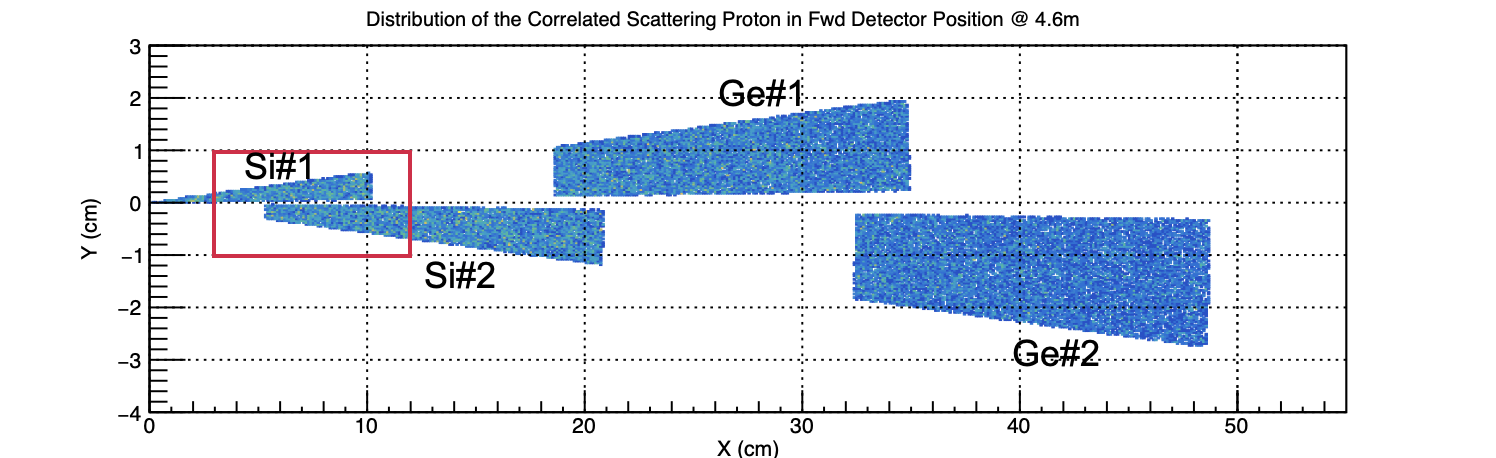
\includegraphics[width=0.45\textwidth]{./fwd_acceptance.png}
  \caption{
    Distribution of hit position of the forward scattered particle on a plane at
    $z=\SI{4.6}{\m}$ that is coincident with the recoil particle hitting one of
    the four recoil sensors.
    The red square indicates the fiducial volume of the forward scintillators.
    The vertical dashed line indicates the hit positions with $|t| = \SI{0.001}{\tmom}$.
    The results are from the simulation of \SI{2.2}{\momentum}
    $pp$ elastic scattering: a) ideal point-like beam; b) $\SI{10}{\mm}\times\SI{10}{\mm}$ box beam profile.
    }
  \label{fig:forward_acceptance}
\end{figure}
Based on the simulation study, the current width of the forward detector
scintillator only guarantees coincidences between the forward detector and the
recoil detector for $|t| < \SI{0.001}{\tmom}$ at the COSY beam momentum range if the beam spot has a diameter smaller than \SI{7}{\mm}.
% The actual coverage can to be extracted in the data analyis, see Sec. \ref{sec:result}.

The scintillator bar is read out by the combination of a tapered light guide, a silicone pad and a
photomultiplier tube (Hamamatsu H6900 \cite{hamamatsu}), as shown in Fig. \ref{fig:forward_module} (a).
Each detector module is integrated into a forward chamber flange for usage
in the ultra-high vacuum.
To meet the vacuum requirements inside the beam pipe, the following designs are implemented:
\begin{enumerate}
\item only the light guide and the scintillator are installed inside the forward chamber, the light guide is glued on the open port of the flange as a feedthrough;
\item no wrapping and painting material is on the surface of the scintillator, the
  surface is polished to increase the light collection efficiency;
\item a thin aluminum tube of \SI{100}{\micro\meter} thickness is used as
  the light shield to prevent light cross-talk between the scintillators, the tube is screwed on the flange, see Fig. \ref{fig:forward_module} (b);
\item two small holes, which are aligned to the thin side of the scintillator, are opened on the wall of the aluminum tube to speed up vacuum pumping, see Fig. \ref{fig:forward_module} (c).
\end{enumerate}
Other components such as the silicone pad, the PMT and the PMT base are
installed inside a light-tight case outside of the vacuum volume, as shown in Fig. \ref{fig:forward_module} (c).
\begin{figure}[htbp]
  \centering
  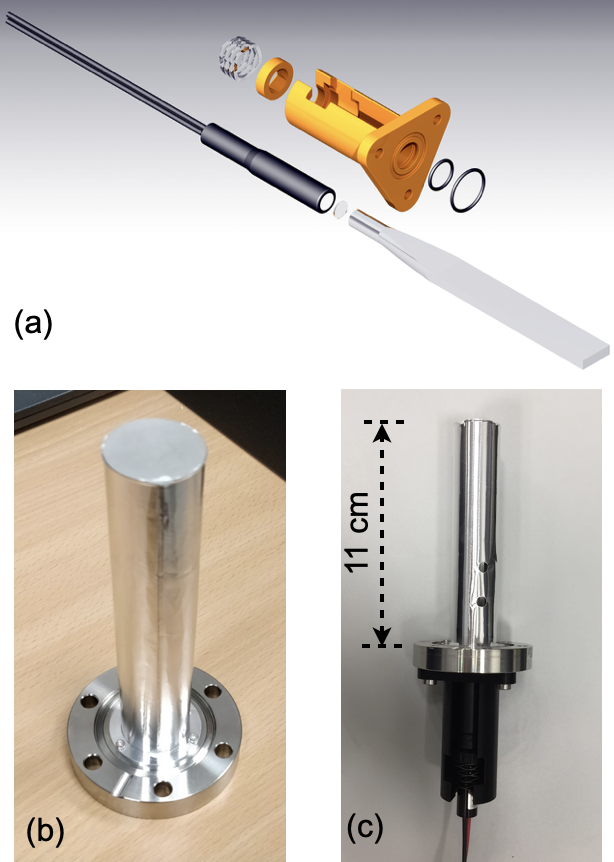
\includegraphics[width=0.32\textwidth]{./forward_module.png}
  \caption{(a) The CAD model of the assembly of a forward detector module; (b) The
    aluminum tube is fixed on the flange inside the vacuum volume; (c) One forward detector module after complete assembly.}
  \label{fig:forward_module}
\end{figure}

Due to the large gain of the PMT, no front-end electronics are needed for the readout of the forward detector.
The output signal from H6900 is split into two branches: one is fed to a
constant fraction discriminator for the time information extraction; the other
is used for the charge measurement.
The modules were tested in the laboratory using cosmic rays before installation.
In each test, two modules were arranged in a cross layout so that only vertical
cosmic rays were selected.
% A typical MIP spectrum obtained by the forward detector module is shown in Fig. \ref{fig:forward_mip}. 
The minimum ionizing particle (MIP) peak is well separated from the pedestal
noise, with the signal to noise ratio (SNR) larger than 50.
The timing resolution of a single module ($\sigma_{module}$) can be deduced from
the time difference distribution of the two modules being tested by $\sigma_{module}=\sigma_{diff}/\sqrt{2}$.
Typical timing resolutions (FWHM) is about \SI{360}{\pico\second}, which is
sufficient for the KOALA experiment.

\section{Data acquisition system}
\label{sec:daq}
\begin{figure*}[bt]
  \centering
  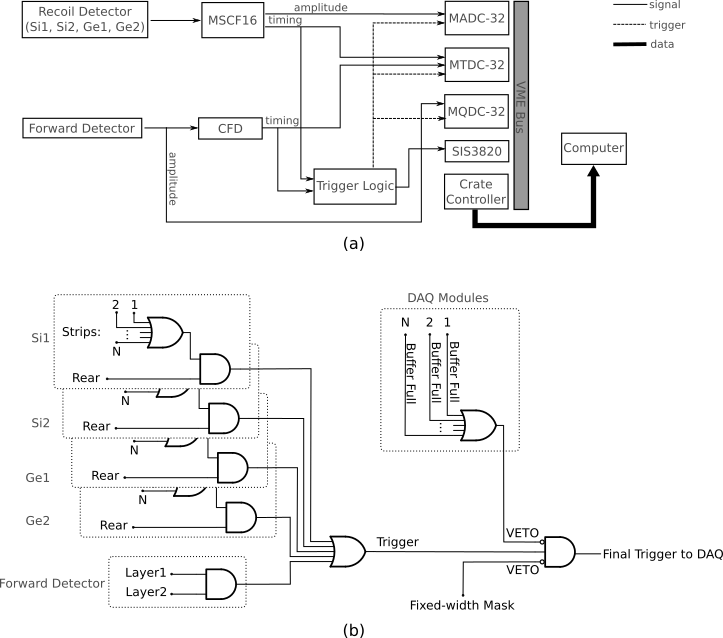
\includegraphics[width=0.75\textwidth]{./daq_scheme.png}
  \caption{a) Block diagram of the KOALA DAQ system; b) Schematic overview of
    the trigger logic design.}
  \label{fig:trigger_logic}
\end{figure*}
The event rate of $pp$ elastic scattering at COSY is about \SI[per-mode=power]{e2}{\per\second}.
At HESR, the estimated rate for $\bar{p}p$ elastic scattering is about a factor of 2 lower.
A single-crate data acquisition system based on the VME bus was developed for the KOALA experiment.
Multiple types of digitization modules produced by Mesytec \cite{mesytec} are
used in this system, see Fig. \ref{fig:trigger_logic} (a).
For the recoil detector, the amplitude signal from MSCF16 is digitized by a
peak-sensing ADC module MADC-32.
MADC-32 has a 13-bit dynamic range with \SI{12.5}{\micro\second} conversion time.
For the forward detector, the pulses from the PMTs are directly fed into a QDC
module MQDC-32 for the charge measurement.
MQDC-32 has a dynamic range of \SI{500}{\pico\coulomb} with 12-bit resolution
and \SI{250}{\nano\second} conversion time.
The timing information from both the recoil and forward detectors is recorded
by a TDC module MTDC-32 with \SI{32}{\pico\second} resolution.
MTDC-32 modules are configured to work in the Start-Stop mode, with the DAQ
trigger signal serving as the common start.
A multi-channel scalar SIS3820 \cite{sis} is also integrated to record
the following key count rates: 1) count rates of the four pairs of the forward detector for beam position monitoring; 2) count rates of the overlapping regions of the recoil detector for asymmetry correction; 3) count rates of the input trigger for DAQ efficiency correction.

% The acceptance of the forward detector only covers a small part of the recoil detector sensors.
% To record the elastic scattering events from the whole range of the recoil angle
% covered by the recoil detector,
The KOALA setup adopts a self-triggering scheme for the trigger logic design.
Each sensor of the recoil detector and the X arm of the forward detector works independently and generates its own trigger. 
The final trigger to the DAQ is a common OR of all sub-detectors, as shown in
Fig. \ref{fig:trigger_logic} (b).
The trigger from the recoil detector sensor is generated by a coincidence between the front-side strips and the rear-side plane, 
and the trigger from the forward detector arm is generated by a coincidence between the two modules in the pair.
% In this way, the rate of the false hits generated by electronic noise can be minimized.
Both elastic and inelastic scattering events are recorded in this trigger
design, and the coincidence between the recoil sensor and the forward detector
is carried out in the offline analysis.

Fast readout of the recorded event is crucial for a self-triggered DAQ system.
The asynchronous readout mechanism combined with VME CBLT block read mode is adopted to increase the data throughput.
The digitization modules used in the KOALA setup have an event buffer with a size
larger than \SI{32}{\kibi\byte}.
Digitized events are stored in this buffer before readout, so that the module is
available to digitize the next event without further dead time.
Events will not be readout until the buffer is nearly full.
On the other hand, since the cross section is much higher at smaller recoil
angles, the module buffer for these channels saturates faster than others.
These modules may miss new events, while others might not, generating a systematic bias.
To overcome this potential bias, the buffer-full signal from each module is added to the
trigger logic as a \texttt{VETO}, as shown in Fig. \ref{fig:trigger_logic}.

The need for event synchronization arises naturally when using the asynchronous
readout mode.
The event synchronization is imposed at the hardware-level by adding a fixed-width mask gate into the trigger logic as \texttt{VETO}, see Fig. \ref{fig:trigger_logic}.
The width of the mask gate should be larger than the maximum dead time of all modules.
In this way, the events are effectively synchronized sequentially. 
% The digitization modules used in KOALA have different dead time, especially between MADC-32 and MTDC-32.
% An event recorded by a fast module may be missed by a slow module. This creates un-synchronous event structure, which makes the sequential event data assembling impossible. 
% Timestamp-based synchronization is used to solve this problem.
% The modules in the system have a 30-bit counter for recording the timestamp from
% the clock signal distributed by a central source.
% The source could be either the VME built-in clock (\SI{16}{\MHz}) or an external clock
% (lower than \SI{75}{\MHz}).
% Currently, the built-in clock of VME backplane bus is used. 
% Based on this timestamp, event synchronization is achieved offline.
% The other option is adding a fixed-width mask gate into the trigger logic as \texttt{VETO}, see Fig. \ref{fig:trigger_logic}.
% The width of the mask gate should be larger than the maximum dead time of all modules.
% In this way, the events are effectively synchronized sequentially. 
% However, this method reduces the DAQ efficiency significantly in a high trigger-rate
% environment.
% Due to self-triggering design, this may bring trigger efficiency biases between different sensors of the
% recoil detector if different noise triggering level exists in each sensor,
% see Sec. \ref{sec:conclusion}.

% \raggedright
A dedicated DAQ software called KoalaEms is also developed for the KOALA experiment.
KoalaEms is a fork of the EMS software \cite{ems}, which is a highly flexible DAQ software framework developed for various experiments at COSY.
Support for the VME controller (SIS3100 \cite{sis}) is integrated and a new
component of the online monitoring is added.
The architecture of KoalaEms is shown in Fig. \ref{fig:koalaems}.
\begin{figure}[h]
  \centering
  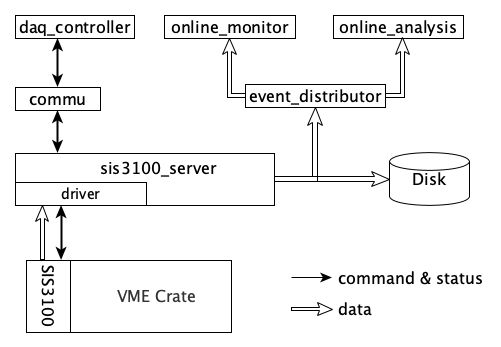
\includegraphics[width=0.45\textwidth]{./koalaems_deployment.png}
  \caption{Schematic overview of the design of KoalaEms.}
  \label{fig:koalaems}
\end{figure}
The interface to the DAQ is implemented as \texttt{sis3100\textunderscore server}, the host of which
connects to SIS3100 by an optical link.
The control and status information from/to the GUI \texttt{daq\textunderscore controller} is mediated by a component called \texttt{commu}.
The data flow from the VME crate is split into two branches:
\begin{enumerate*}[label=(\roman*)]
\item \texttt{data\textunderscore out\textunderscore di\allowbreak sk}: save the raw data onto disk;
\item \texttt{data\textunderscore out\textunderscore stream}: stream out to \texttt{event\textunderscore distributor}.
\end{enumerate*}
The data stream is forwarded by \texttt{event\textunderscore distributor} to various consumption hosts for usages like online monitoring and online analysis.
Both \texttt{commu} and \texttt{event\textunderscore distributor} support socket connection and \texttt{event\textunderscore distributor} also supports multiplexing streaming.
All components shown in Fig. \ref{fig:koalaems} can be hosted in different PCs
and a new consumption host to the data stream can be integrated whenever needed.
% \justify

\section{Software framework}
\label{sec:software}

A software framework called KoalaSoft has been developed for the simulation, calibration, reconstruction and analysis jobs of the KOALA experiment.
It is built upon the FairRoot \cite{fairroot} framework, which implements a
simulation environment based on the VMC \cite{vmc} library and an analysis
environment based on ROOT's task concept \cite{root}.
The components stack of KoalaSoft is shown in Fig. \ref{fig:koalasoft}.

\begin{figure}[htbp]
  \centering
  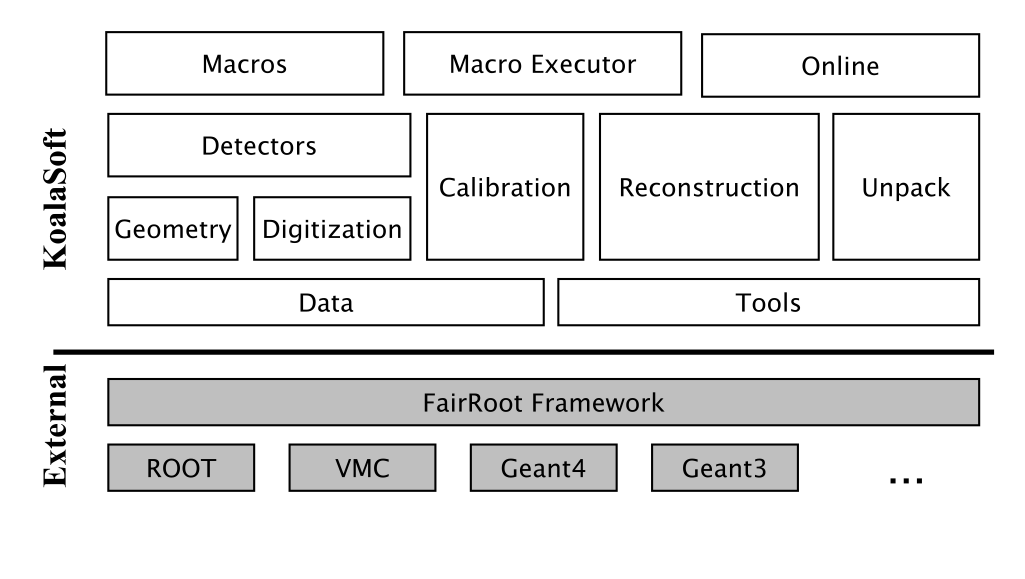
\includegraphics[width=0.48\textwidth]{./koalasoft_components.png}
  \caption{Overview of the KoalaSoft components.}
  \label{fig:koalasoft}
\end{figure}

\textit{FairRoot} provides an integrated and unified interface to the underlying facility
packages such as \textit{ROOT}, \textit{VMC}, \textit{Geant3}, \textit{Geant4} etc.
% By using VMC it is possible to choose between Geant3 or Geant4 as the simulation engine without changing other components in KoalaSoft.
The \textit{Data} component provides all the data types needed for the running
of KoalaSoft in memory and for the persistent storage in the disk ROOT files.
The \textit{Tools} component provides the common tool classes needed by other
components, such as the detector geometry management in the data analaysis and
the channel number encoding and decoding.
The \textit{Geometry} component provides the scripts  used to generate the KOALA detector models.
Geometry models are implemented using the TGeo library of ROOT.
The \textit{Detectors} component provides the functionality needed in the
detector simulation.
Analysis jobs after the simulation are divided into multiple smaller steps, each of which is
then implemented as a single FairRoot task in KoalaSoft.
Tasks can be chained together later in a ROOT macro to compose a full job. 
Dedicated tasks for commonly used jobs are stored together in KoalaSoft such as
\textit{Digitization}, \textit{Calibration} and \textit{Reconstructionare} in
Fig. \ref{fig:koalasoft}.
ROOT macros are adopted as the usage interface for the end user using KoalaSoft.
Macros for common jobs are pre-configured and stored in the \textit{Macros} component.
Additionally, a binary macro executor is provided with the \textit{Macro
  Executor} to run jobs directly from the command line. This component is useful in batch processing.

The same chain of tasks can be used for the analysis of both the simulated data
and the raw data from the DAQ in KoalaSoft.
This is accomplished by the \textit{Unpack} component, which can decode and transform the raw binary data into the same format as the output from simulation jobs.
Thus, algorithms developed, tested and verified using simulated data can be applied to experimental data seamlessly.
This saves much effort in the development and maintenance of algorithms.
Both the offline disk data and the online streaming data are correctly handled
by \textit{Unpack}.
An online monitoring program is developed based on \textit{Unpack} and provided
in the \textit{Online} component.

\section{Calibration of the recoil detector}
\label{sec:calibration}

\subsection{Energy calibration}
\label{sec:energy_calibration}

% Precise measurement of energy deposit in the recoil detector is critical for the
% identification of elastic scattering events as well as the calculation of the recoil angle.
\(^{239}Pu\), \(^{244}Cm\), \(^{241}Am\), with main $\alpha$ decay energies
of \SIlist{5156.59;5804.83;5485.56}{\keV}, respectively \cite{nuclear_data}, are
used for the energy calibration of the recoil detector.
Decays with smaller branching ratios are also utilized if they are well separated from the main peaks.
The average energy resolutions of the silicon and germanium
sensor strips are approximately \SI{20}{\keV} and \SI{30}{\keV} (FWHM)
respectively, for alpha particles with about \SI{5.8}{\MeV} from the $^{244}Cm$ source.

Two aspects need special consideration in the calibration.
First off, the recoil sensors have a thin protective layer on the surface and this
causes energy loss before particles enter the fiducial volume of the sensor.
The thickness of the protection layer has been determined in the laboratory
\cite{recoil_article} and the energy loss of $\alpha$ particles can be estimated
with the LISE++ program \cite{LISE}.
The estimated energy losses of $\alpha$ particles incident at a normal angle to
the detector surface are listed in Tab. \ref{tab:dead_layer} for each sensor.
The effective energy deposit in the fiducial volume is then corrected based on the recoil angle, where each strip is located.
\begin{table}[h!]
  \centering
  \caption{Energy loss (\si{\keV}) in the protection layer for an alpha particle
    at nominal incidence angle.}
  \label{tab:dead_layer}
  \begin{tabular}{cccccc}
    \hline
    \(E_{\alpha} (keV)\) & \(\Delta E_{Si1}\) & \(\Delta E_{Si2}\) & \(\Delta E_{Ge1}\) & \(\Delta E_{Ge2}\) \\
    \hline
    5156.59 & 11.51 & 11.51 & 110.00 & 111.00 \\
    5485.56 & 11.01 & 11.01 & 105.00 & 106.00 \\
    5804.83 & 10.52 & 10.52 & 99.00  & 100.00 \\
    \hline
  \end{tabular}
\end{table}

Secondly, the gain setting of each readout channel is optimized for the energy range covered by the corresponding strip.
The gain difference varies by up to a factor $\mathtt{\sim}$10.
% Thus, the resolution is worse at large recoil angles than at small angles, as shown in Fig. \ref{fig:alpha_spectrum}.
% The minor decay modes can't be recognized in Fig. \ref{fig:alpha_spectrum} (a), while they are clearly seen in Fig. \ref{fig:alpha_spectrum} (b).
Thus, the energy resolution is better at small recoil angels than at large angles.
The recorded $\alpha$ energy spectra by one channel close to the IP and one
channel close to the far edge of the recoil detector are shown in Fig. \ref{fig:alpha_spectrum}.
The minor decay modes are clearly seen with a large gain setting (the upper
frame in Fig. \ref{fig:alpha_spectrum}), while they can not be recognized with a
smaller gain setting (the bottom frame in Fig. \ref{fig:alpha_spectrum}).
The worse resolution brings larger uncertainty in the calibration, since only three energy points can be used.
\begin{figure}[bht!]
  \centering
  % 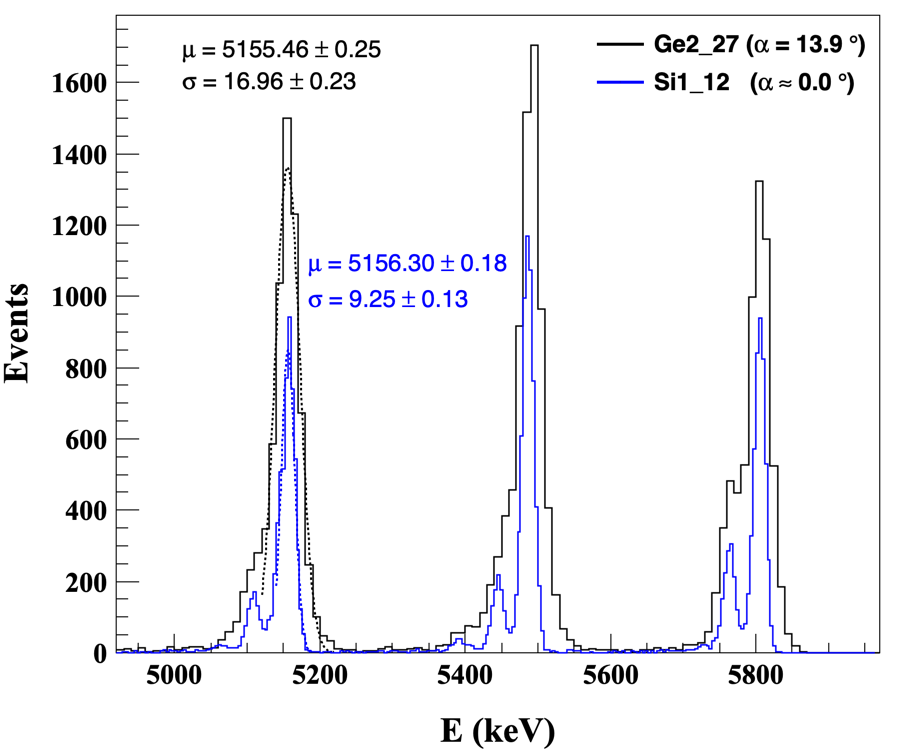
\includegraphics[width=0.45\textwidth]{./alpha_comparison_corrected_fit.png}
  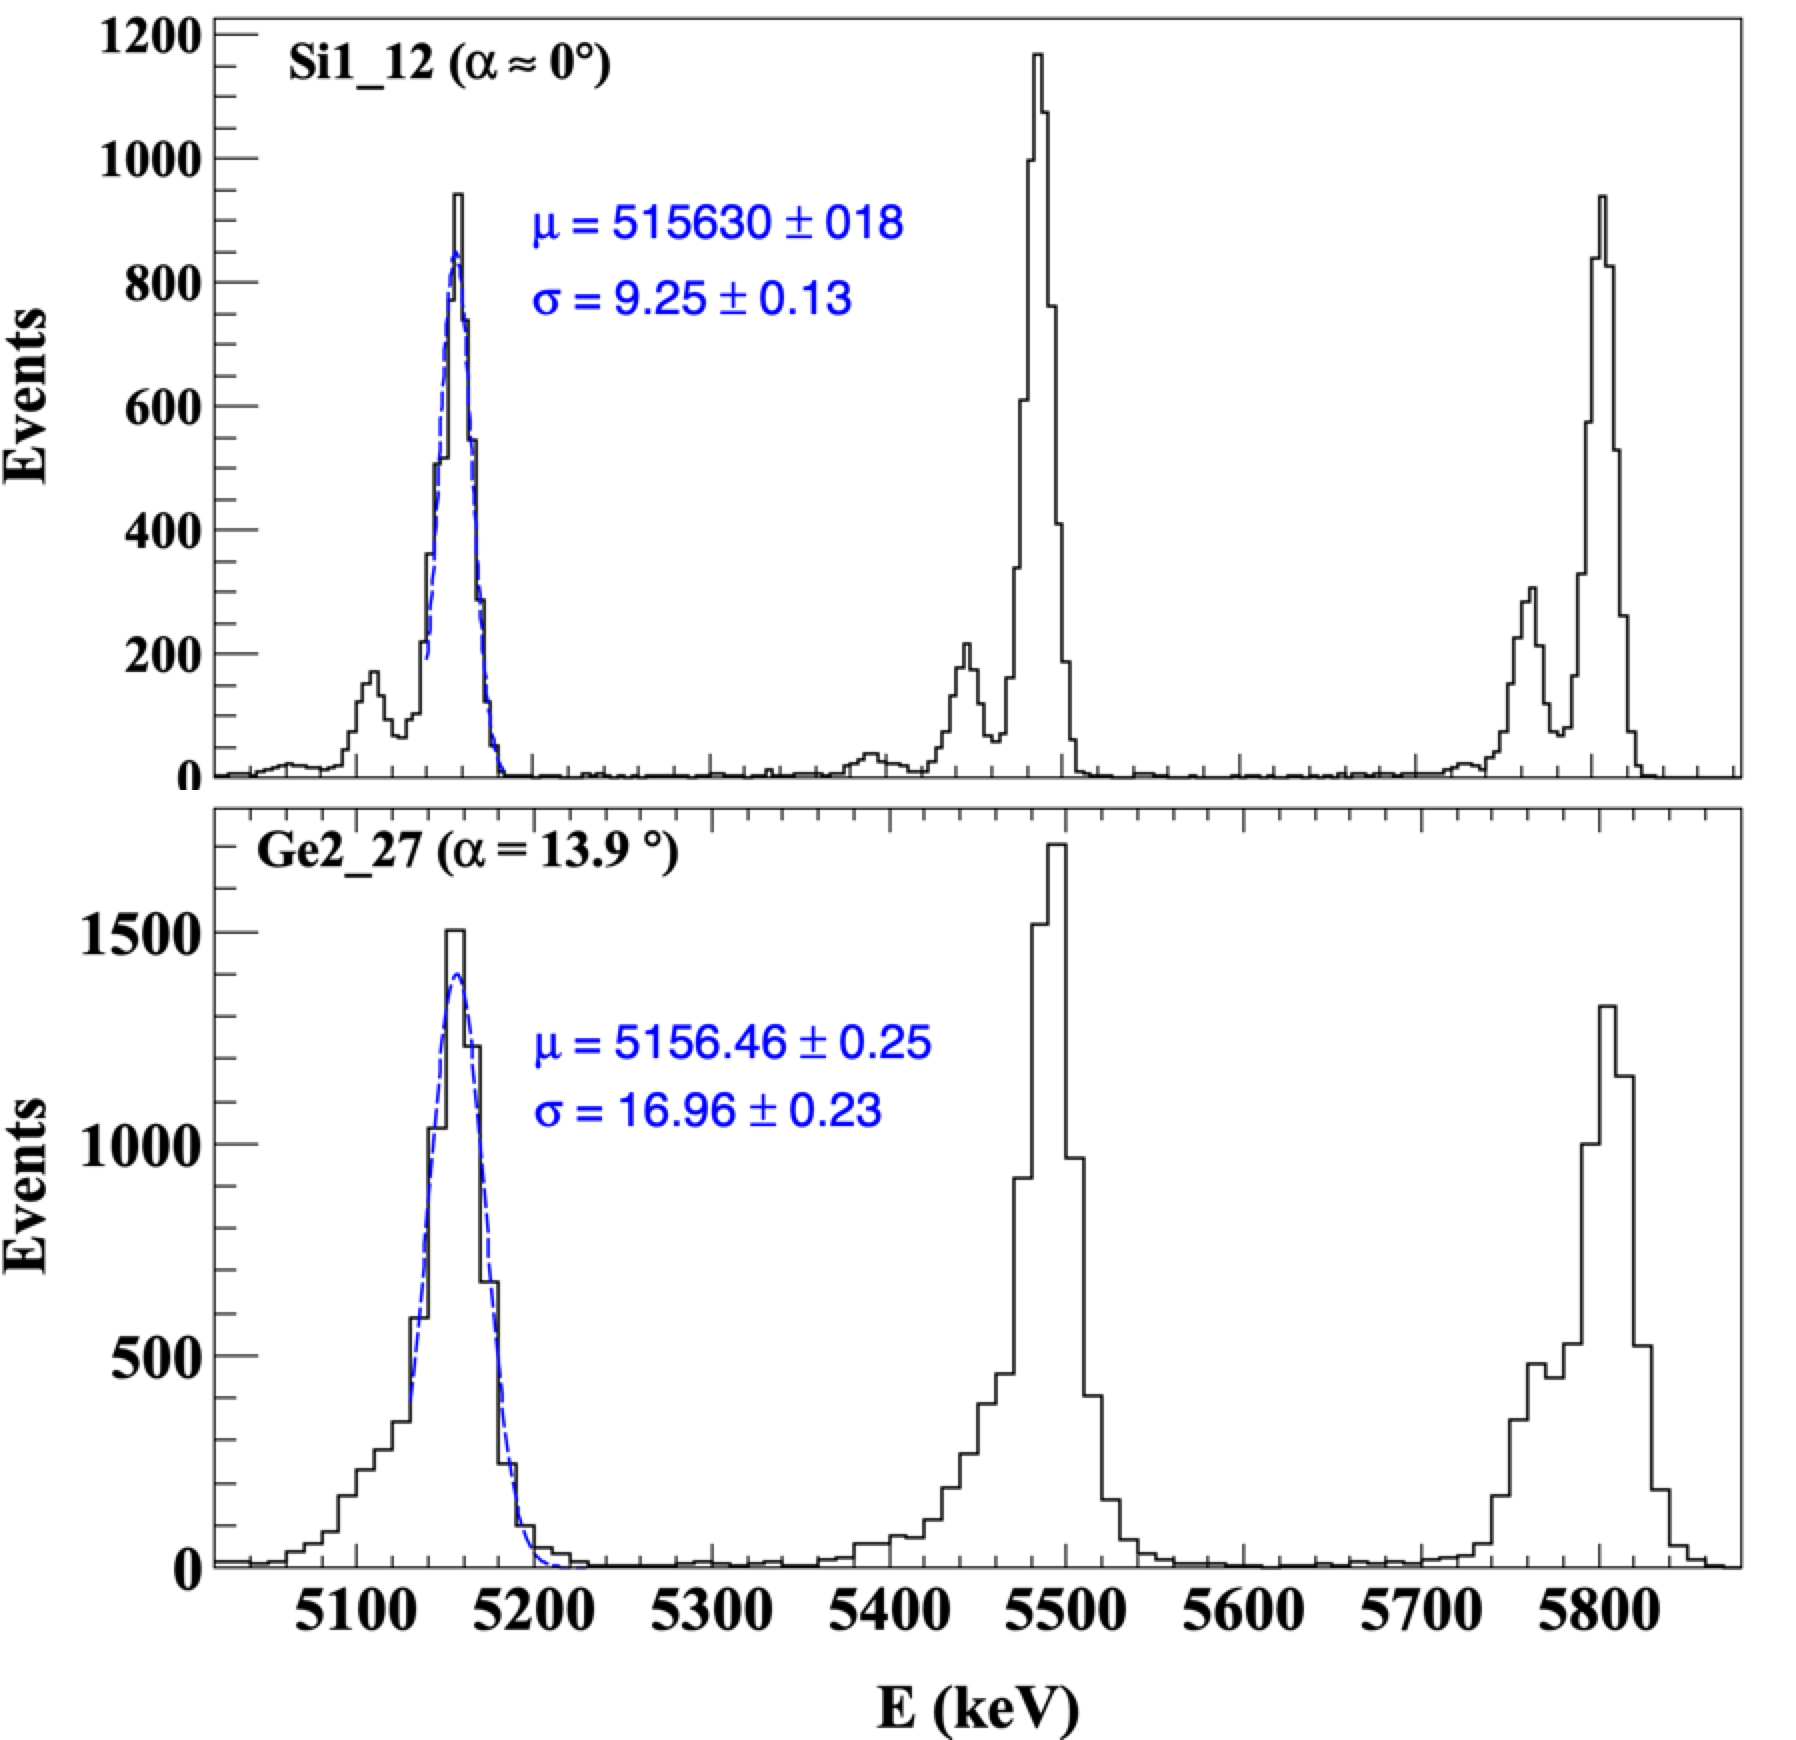
\includegraphics[width=0.45\textwidth]{./alpha_comparison_corrected_fit_separate.png}
  \caption{Energy spectra of \(\alpha\) sources for two channels at small (up)
    and large (down) recoil angles. The main peak from $^{239}Pu$ at
    \SI{5156.59}{\keV} in each spectrum has been fit with a Gaussian.}
  \label{fig:alpha_spectrum}
\end{figure}

To minimize this uncertainty, a common gain setting is set for all channels that optimizes the separation of the \(\alpha\) peaks.
The calibration is carried out indirectly as follows:
\begin{enumerate}
\item \(\alpha\) source calibration is carried out under the common gain setting;
\item the linearity curves at both the common gain and the so-called beam gain
  setting used in the experiment are calibrated using the pulse generator ORTEC Model 419;
\item the $\alpha$ peak at the beam gain setting is then deduced
  from the linearity curve at a pulser amplitude which generates the same peak
  value as the $\alpha$ source when using the common gain setting;
\item the peak responses are fit linearly against the corresponding $\alpha$ energies
  to get the calibration parameters.
\end{enumerate}
The readout electronics of the recoil detector have a good linearity in both common gain and beam gain settings.
Fig. \ref{fig:electronic_linearity} shows the quadratic fit results to the linearity curves for a readout channel of Ge2.
\begin{figure}[b!]
  \centering
  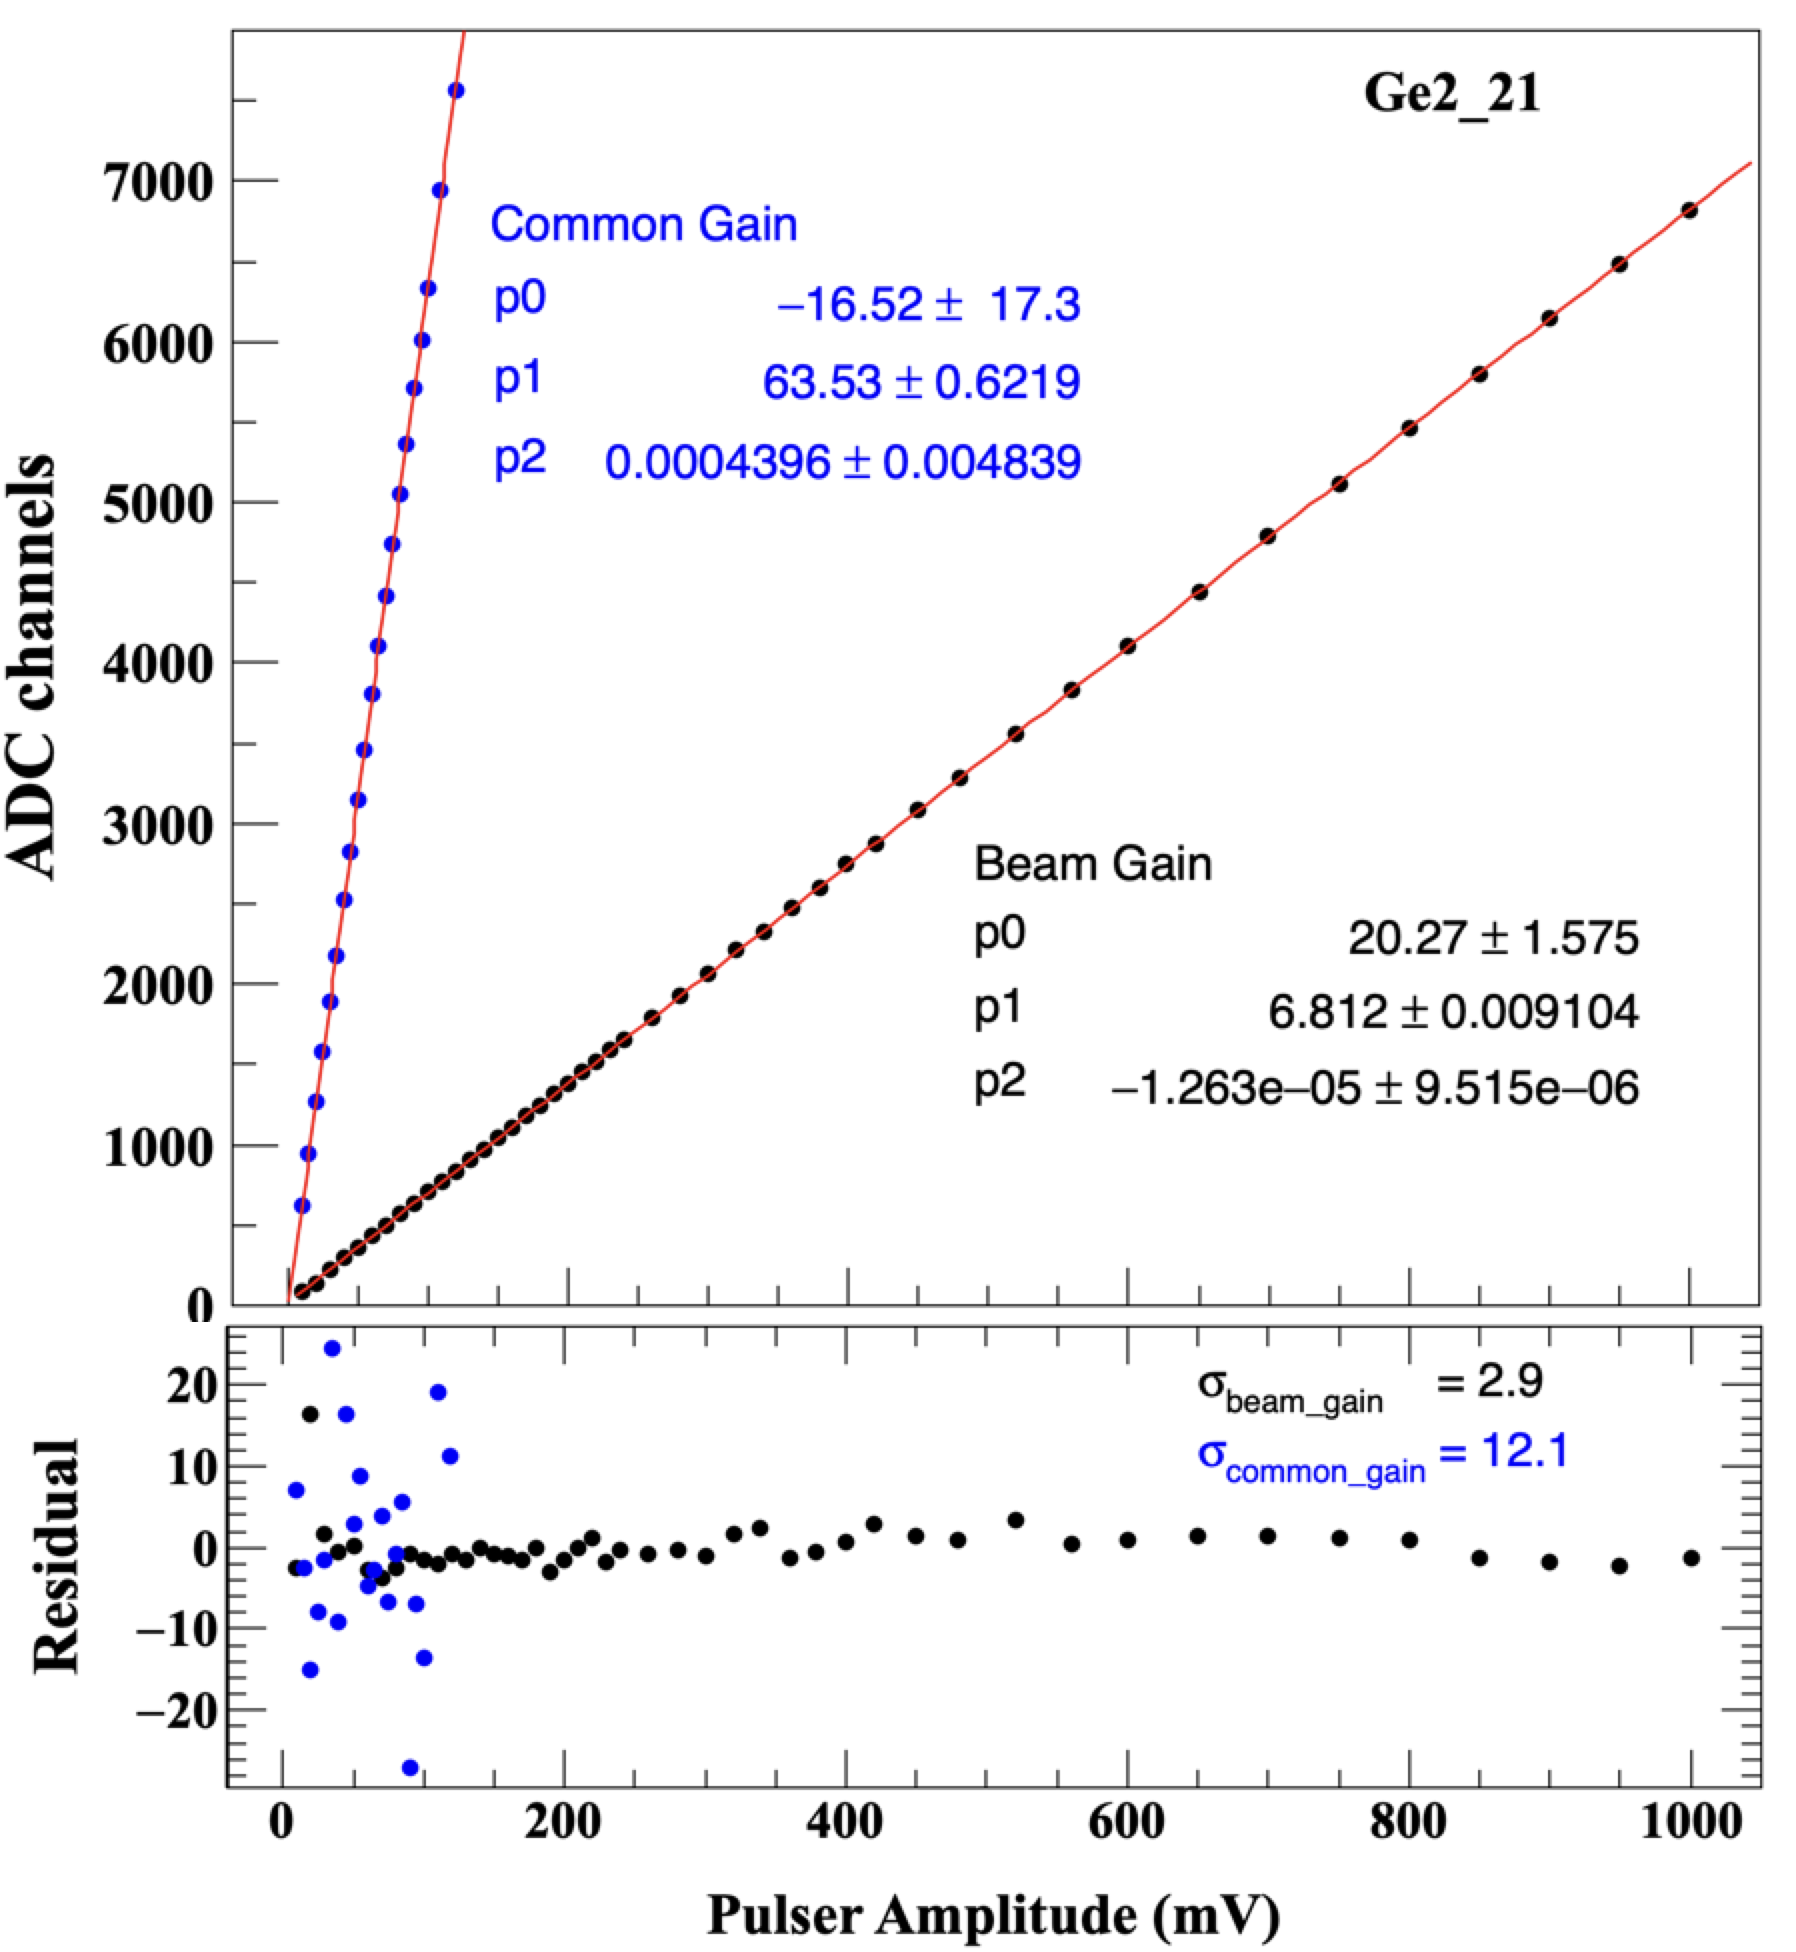
\includegraphics[width=0.45\textwidth]{./linearity_quadratic_residual.png}
  \caption{The results of a quadratic fit to the linearity curves of a recoil
    detector channel. The bottom frame shows the residuals between the data
    points and the linear part of the quadratic function.}
  \label{fig:electronic_linearity}
\end{figure}
In both cases, the quadratic terms are negligibly small and the residuals
between the measurement data points and the linear part have small dispersions
($\sigma=\SI{2.9}{channels}$ for the beam gain setting, $\sigma=\SI{12.5}{channels}$ for the common gain setting).
Thus, linear fitting is adopted in all the calibration steps.
% Due to the good linearity of the readout electronics in both common gain
% and beam gain setting (see Fig. \ref{fig:electronic_linearity}), this indirect
% method does not bring in extra systematic bias.
The fitting parameters from the last step are used to convert ADC channel into
energy value in the reconstruction.
% The achieved precsion of the calibration is about \SI{0.12}{\percent}.

\subsection{Alignment}
\label{sec:alignment}

% During installation, the position of the KOALA setup was adjusted accurately based on the
% coordinate system of COSY using a laser precisioning system.
During installation, the position of the KOALA setup was adjusted to a precision
of \SI{0.1}{\mm} relative to the COSY coordinate system by using a laser positioning system.
However, the relative misalignment between the recoil sensors can't be
determined in this way because they are mounted together on a common sensor holder.
On the other hand, the exact location of the IP needs to be determined for each experiment since
it may vary with the operation conditions of the cluster jet target.
Thus, an alignment based on the experimental data is needed to accurately deduce the recoil angle of the elastic scattering events.

Due to the layout of the recoil sensors, only the alignment along
the beam axis, \textit{i.e.}, Z-axis in the COSY coordinate system, is necessary.
The alignment parameter for each sensor is determined as follows:
\begin{enumerate}
\item the peak energy of elastic scattering events on each strip is extracted
  (see Sec. \ref{sec:recoil_performance} and Sec. \ref{sec:tofe_selection}) and converted to a calculated position along the beam axis based on the elastic
  scattering kinematics;
\item for strips from the same sensor, the difference between the calculated
  position and the nominal position of each strip from the ideal geometry model is filled into the same histogram, as shown in Fig. \ref{fig:alignment};
\item the peak region in the histogram is fit with a Gaussian to get the offset
  of each sensor compared to the nominal position.
\end{enumerate}
\begin{figure}[th!]
  \centering
  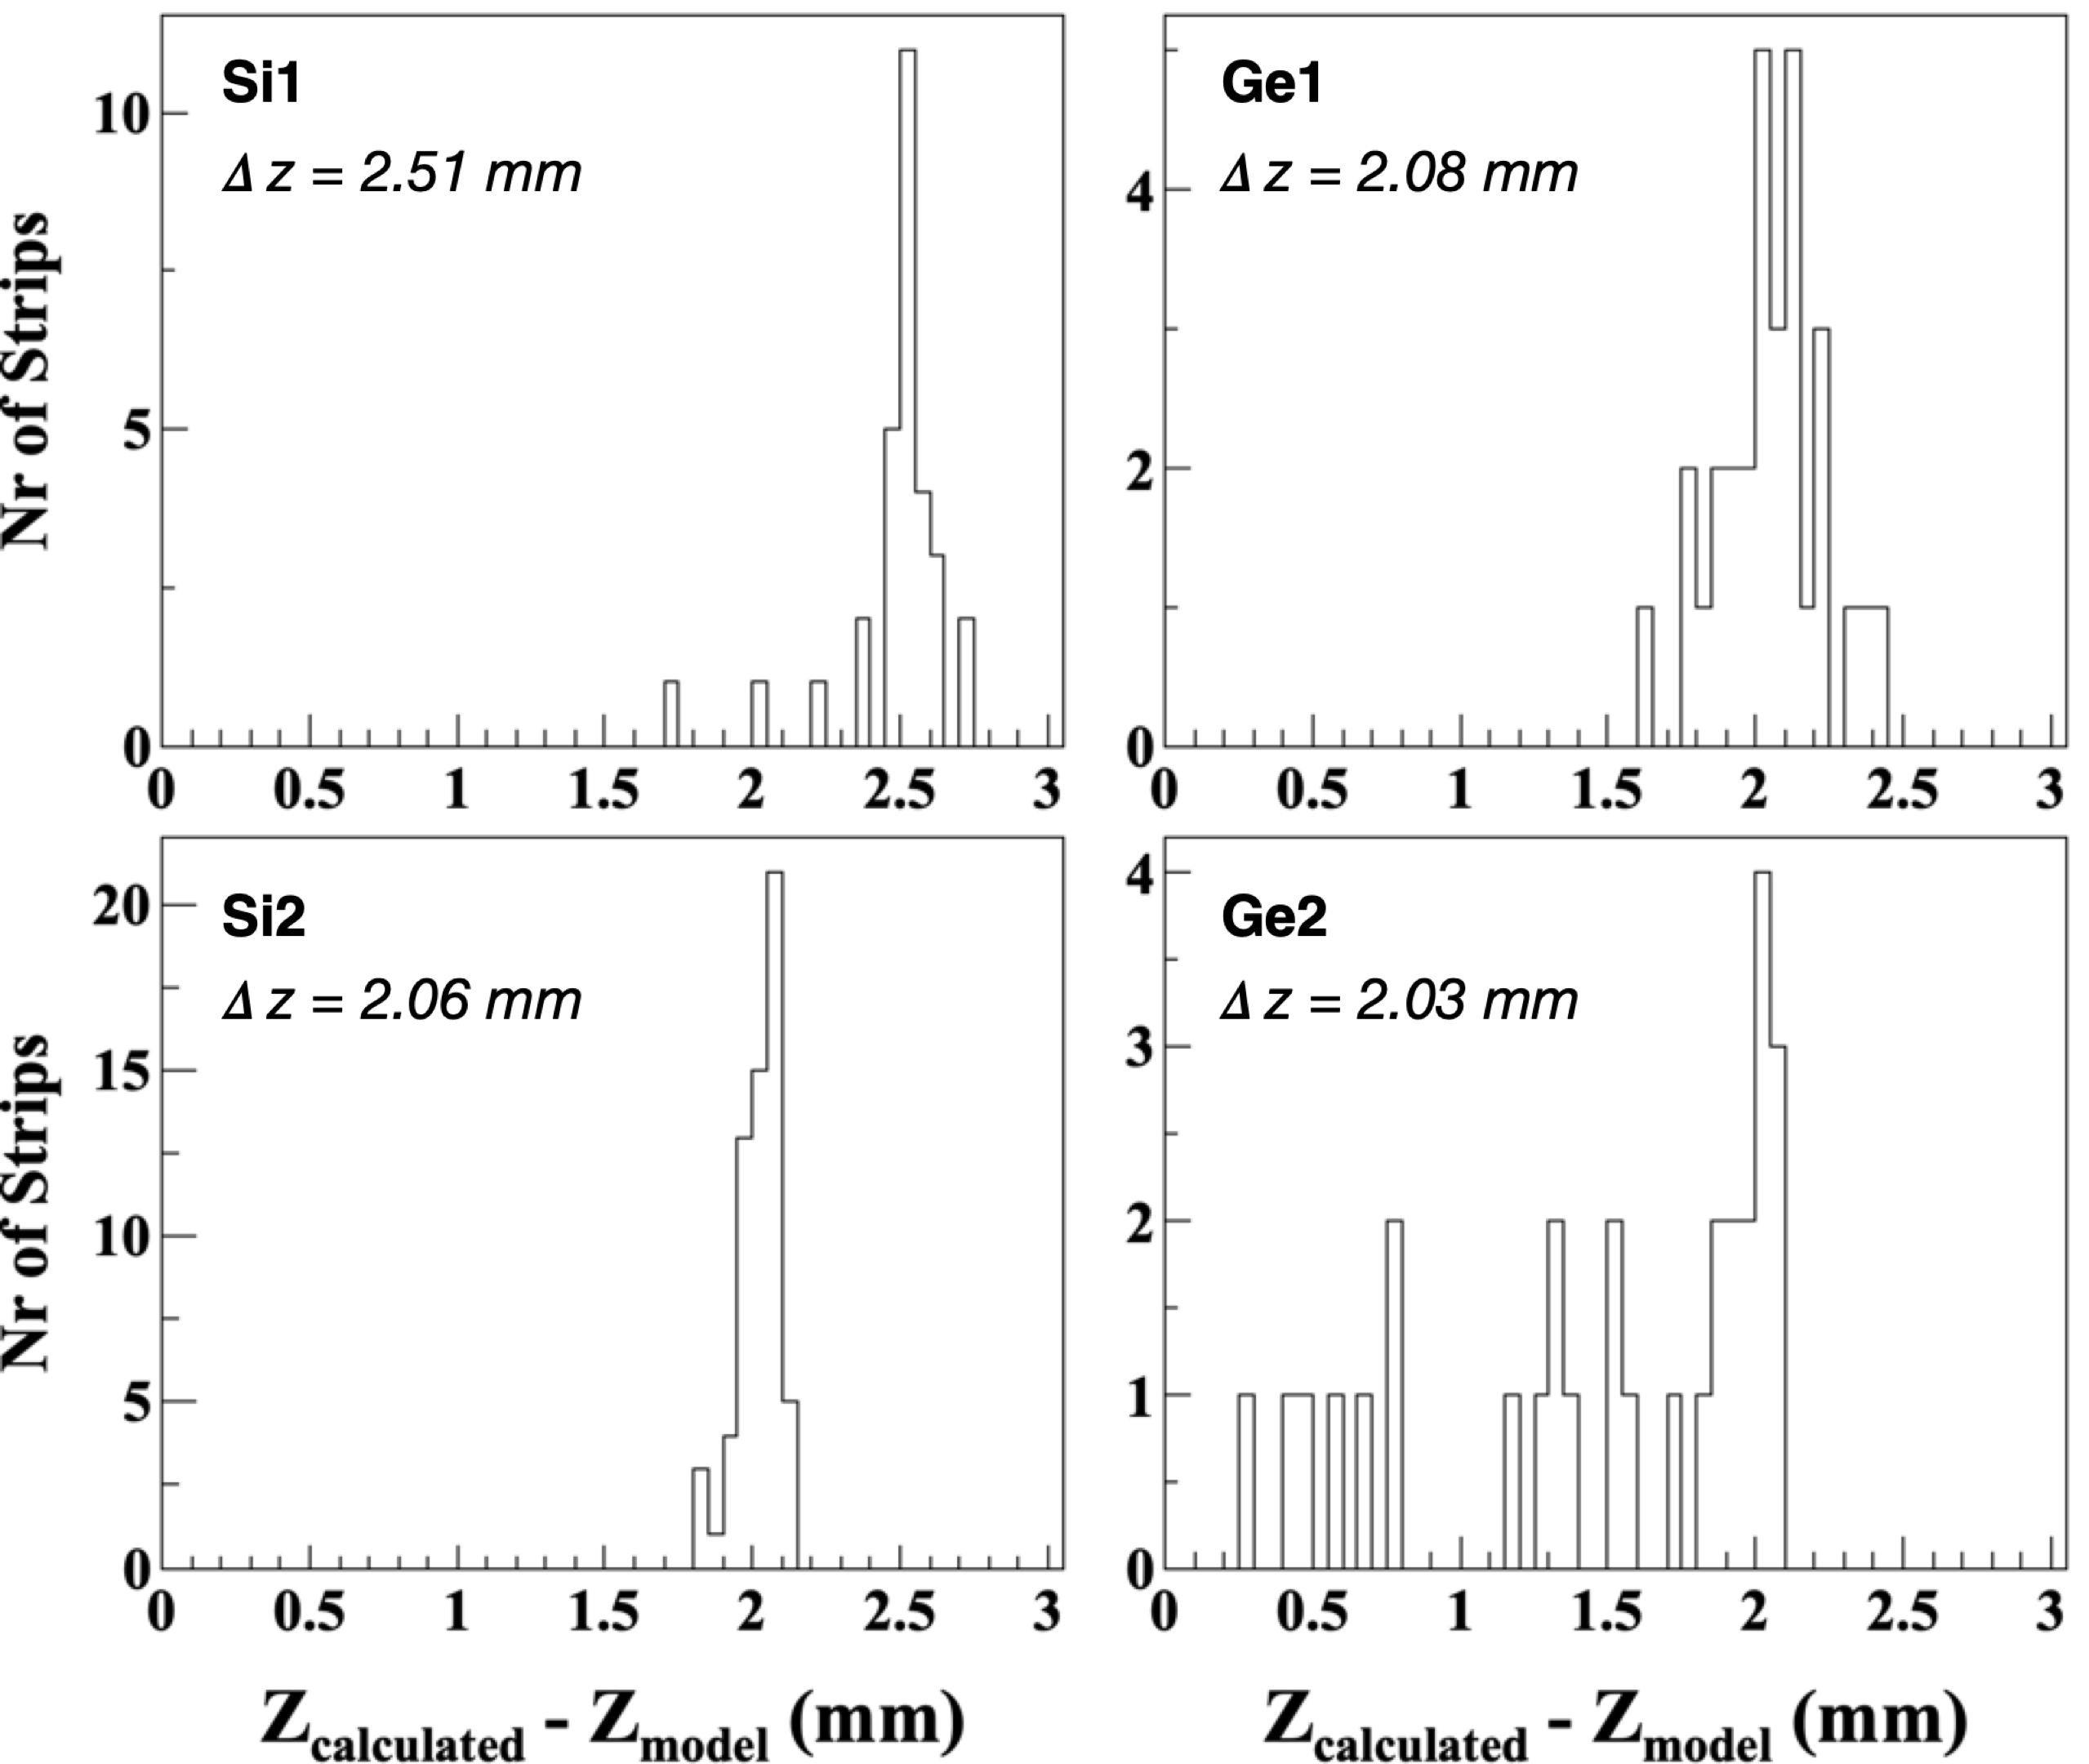
\includegraphics[width=0.45\textwidth]{./alignment_reorder.png}
  \caption{Histograms of the difference between the calculated position from the
    elastic peak energy and the nominal position from the geometry model.
    The obtained alignment parameters are
    \SIlist[list-units=single]{2.51;2.06;2.08;2.03}{\mm} for Si1, Si2, Ge1, Ge2, respectively.
    This result is from the data obtained at $P_{beam} =
    \SI{2.2}{\momentum}$.}
  \label{fig:alignment}
\end{figure}
These offset values are the corresponding alignment parameters that are later applied in the reconstruction.
Thus, the recoil sensors are aligned so that the IP is at the origin of the
laboratory coordinate system and the misalignment between the sensors is
simultaneously corrected.

\subsection{Time walk correction}
\label{sec:timewalk}

Time walk of the leading edge discriminator used in the recoil detector needs to be corrected to optimize the timing resolution.
The calibration of the time-walk effect is carried out with a precision pulse generator (ORTEC Model 419 \cite{ortec}). 
The output of the pulser is split into two branches: one is fed into a constant fraction discriminator to generate the reference time;
the other is connected to the detector channel that is being calibrated. 
By scanning the pulser over a wide range of amplitudes, the time-walk effect is measured.
An example is shown in Fig. \ref{fig:timewalk}, where the result has been fit with \(y=p_0 x^{-1} + p_1\). 
The time walk is corrected by subtracting \(\Delta t = p_0/ADC\) from the measured timing value.
\begin{figure}[htbp]
  \centering
  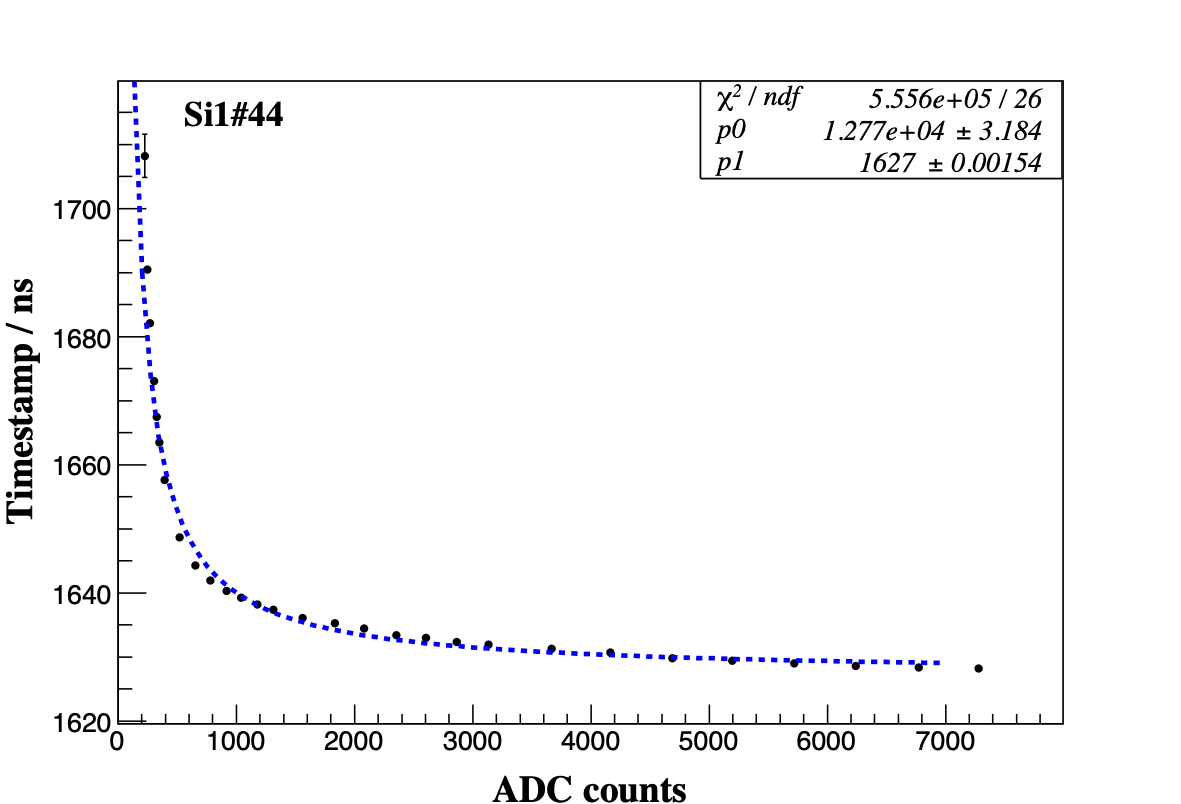
\includegraphics[width=0.45\textwidth]{./timewalk.png}
  \caption{Typical result from the time-walk calilbration, plotted for a single
    strip on the Si1 sensor.}
  \label{fig:timewalk}
\end{figure}

The difference of the fit parameters \(p_1\) indicates the delay time
difference between different channels, which is caused by the signal routing length variation.
These offsets are also corrected in the reconstruction to align the timing from different channels.
% The overall constant is added to account for the time delay between the forward
% detector and the recoil detector.

\section{Clustering}
\label{sec:clustering}

% The primary goal of clustering is to correctly reconstruct the deposited energy.
% Comparing the conventioanl experiment, the identification of the impinging strip of
% the cluster is also critical in the KOALA experiment, so as to correctly
% reconstruct the recoil angle and obtain the correct yield on each strip.

The clustering algorithm combines information from adjacent recoil strips in
order to improve the response function of the sensor to the deposited energy and
hit location of the recoil proton.
This is necessary to optimize the performance of the detector to determine the yield of elastically scattered events as a function of recoil angle.

Clustering is necessary due to following reasons:
\begin{enumerate*}[label=(\roman*)]
\item charge sharing is an intrinsic characteristic of the solid-state strip detector, especially for the tracks that hit the region close to the border between adjacent strips;
\item tracks with large recoil angles may penetrate several strips before stopping.
\end{enumerate*}
The results from the simulation and the beam commissioning both show that more
than \SI{50}{\percent} of the tracks that hit the Ge2 sensor have a hit multiplicity
larger than 1.
The hit multiplicity distributions in the four
recoil sensors are listed in Tab. \ref{tab:multiplicity}.
\begin{table}[htb!]
  \centering
  \caption{Hit multiplicity distributions for the recoil sensors recorded for
    proton beam at $P_{beam} = \SI{2.2}{\momentum}$.}
  \label{tab:multiplicity}
  \begin{tabular}{@{} *{5}{c} @{}}
    \hline
    \headercell{\\Sensor} & \multicolumn{4}{c@{}}{Mutliplicity (\si{\percent})} \\
    \cmidrule(l){2-5} & 1 & 2 & 3 &  4 \\
    \midrule
    Si1 & 95.51 & 4.38 & 0.08 & 0.02 \\
    Si2 & 92.46 & 7.21 & 0.24 & 0.06 \\
    Ge1 & 81.06 & 16.61 & 1.51  & 0.44 \\
    Ge2 & 45.41 & 46.30 & 3.98  & 1.67 \\
    \hline
  \end{tabular}
\end{table}

The clustering algorithm is designed to minimize the noise contribution while
% keeping the low-energy background characteristic as much as possible.
not introducing a selection bias between the low energy and high energy elastic events.
The steps of clustering are as follows:
\begin{enumerate}
\item Determine the noise level $\sigma_{noise}$. An event sample which is
  triggered only by the forward detector is selected.
  The pedestal of the energy spectrum is fit with a Gaussian to extract $\sigma_{noise}$ for each
  readout channel.
  \begin{figure}[b]
    \centering
    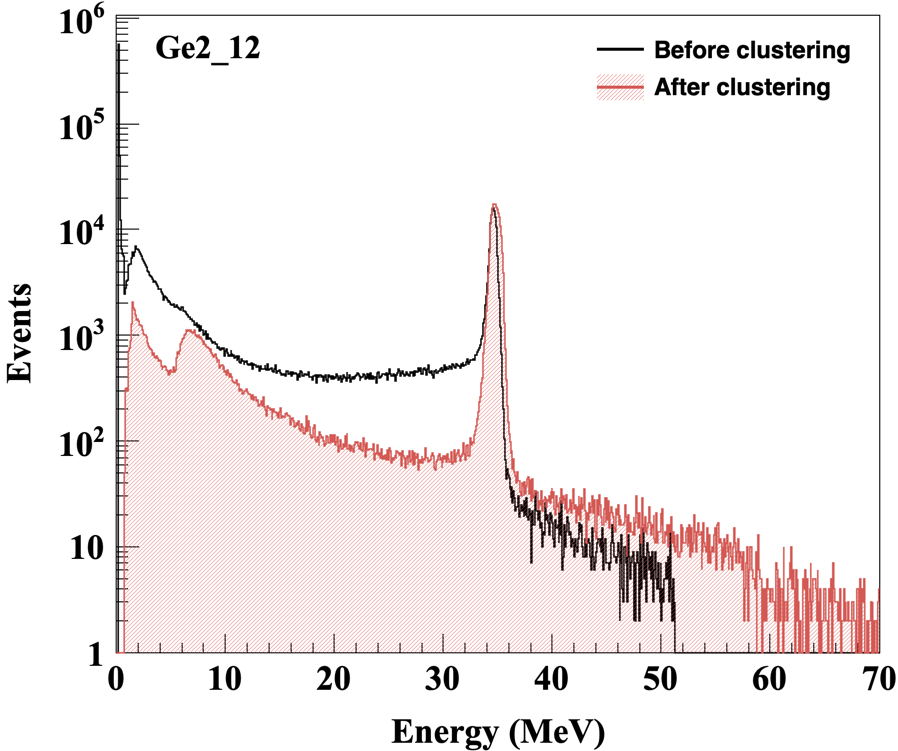
\includegraphics[width=0.45\textwidth]{./clustering.png}
    \caption{The recoil energy spectrum measured by a channel of the Ge2 sensor before (black) and after (red) the clustering.}
    \label{fig:clustering}
  \end{figure}
\item Delete noise hits with an energy below a threshold of $2\sigma_{noise}$.
  % Hits induced by the electronic noise are deleted. A low threshold ($2\sigma_{noise}$) is used in this step.
\item Combine adjacent hits that are above threshold into clusters.
\item Delete noise clusters. The noise level of a cluster with $n$ hits is evaluated as
  $\sigma_{cluster} = \sqrt{\sum_{i=1}^n{(\sigma_{noise}^i)^2}}$, where $\sigma_{noise}^i$ is
  the noise level of the $i_{th}$ strip in the cluster. Clusters with energy lower than $5\sigma_{cluster}$ are considered to be noise-induced and deleted.
\item Delete clusters without a seed hit. The seed hit is defined as the
  hit whose energy is above the trigger threshold of the corresponding readout
  channel. Since a low trigger threshold is used ($\sim\SI{50}{\keV}$), valid clusters need to have at least one seed hit.
\end{enumerate}
The impinging position and impinging time of the cluster are both extracted from the first
hit in the cluster to keep the most accurate information about the recoil angle.

%%%%% integral (pean+- MeV) to get different yield increase, shift of the peak,
%%%%% peak to valley ratio, a table of 3x4 with 6 numbers
\begin{table}[h!]
  \centering
  \caption{Characteristics of the energy spectra in Fig.
    \ref{fig:clustering}. The yield is obtained by integrating a $\pm 1\si{\MeV}$ window around the peak.}
  \label{tab:clustering}
  \begin{tabular}{cccc}
    \hline
    & $E_{peak}(\si{\MeV}$) & Peak-to-Valley & Yield \\
    \hline
    Before & 34.6 & 33  & 148,002 \\
    After  & 34.7 & 234 & 227,033 \\
    \hline
  \end{tabular}
\end{table}
A comparison between the energy spectrum before and after clustering is shown in Fig. \ref{fig:clustering}.
Three characteristics of the energy spectra are also extracted and listed in Tab. \ref{tab:clustering}.
After clustering, a large fraction of the hits in the plateau below the elastic
peak have migrated into the elastic peak.
Multi-hit clusters are now reconstructed under the elastic peak, thus
giving a more accurate determination of the elastic yield on the strip.
The quality of the energy spectrum in terms of peak-to-valley ratio increases from about 33 to about 234.
% The charasteristics of the background shape also show up with two explicit components: 1) a peak which equals MIP's energy loss in the recoil sensors; 2) a smooth decay with a long tail.
The characteristic shape of the background spectrum also shows up more explicitly.
Very noticible is the appearance of a peak at about \SI{7}{\MeV},
which is caused by MIPs (mostly \Pgppm) from inelastic events.
A correct description of the background shape (see Sec.
\ref{sec:recoil_performance}) is only possible after clustering.

\section{Commissioning with proton beam}
\label{sec:result}

Tests were carried out using the proton beam at COSY with momenta of
\SIlist[list-units=single]{2.2;2.4;2.6;3.0}{\momentum}.
% The data analysis procedures of the test beam data are same for all momentums.
In the following, the results from \SI{2.2}{\momentum} are shown as an example.

\subsection{Beam condition}
\label{sec:beam}
The COSY storage ring has a circumference of \SI{184}{\meter}.
To minimize the beam emittance, stochastic cooling \cite{cooling} was applied in
these tests.
The number of protons stored in the ring varied from cycle to cycle between
\SIrange{1.0e10}{2.0e10}, and was measured by a beam current transformer \cite{bct}.
The storage time for a beam cycle in these tests was about \SI{300}{\second}, as shown in Fig. \ref{fig:beam}.
% The cooling reaches the equibilium state after the beginning $1/3$ of the storage cycle.
\begin{figure}[h]
  \centering
  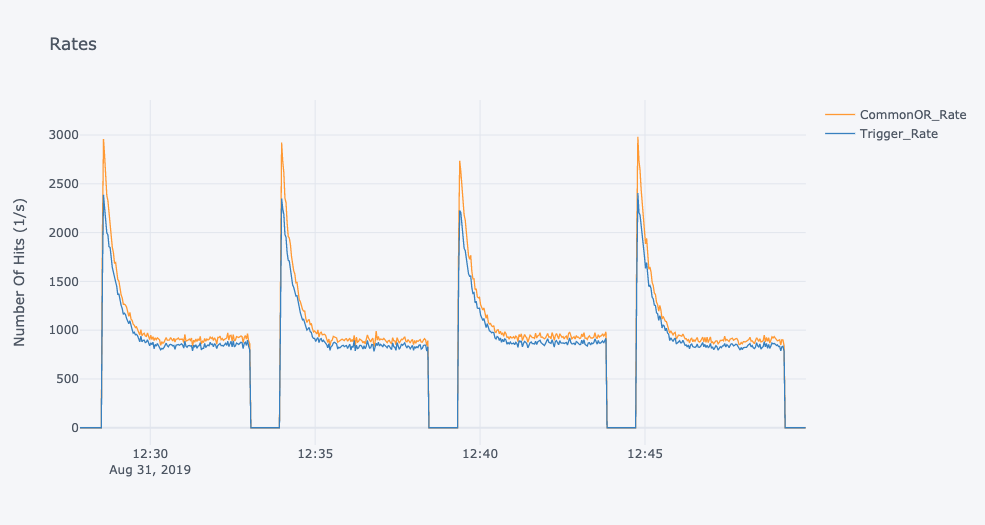
\includegraphics[width=0.45\textwidth]{./daq_efficiency.png}
  \caption{Time variation of the total input trigger rate (red) and the ratio between the accepted and total input trigger rate (blue), which is a direct measure of the DAQ efficiency.}
  \label{fig:beam}
\end{figure}
% During injection cycle, the beam has large emittance and not stable.

The measurements were only performed during the storage cycle, which is signaled by two
gates generated by the COSY control.
One gate is used to protect the PMTs of the forward detector during injection.
It ramps down the high voltage supply \SI{5}{\second} before the end of the
storage cycle and ramps up the high voltage supply \SI{5}{\second} after the start of the storage cycle.
The other gate has a narrower width and is used to control the DAQ system so
that data is not recorded during injection and beam dump.

The DAQ efficiency is seen in Fig. \ref{fig:beam} to significantly depend upon the
instantaneous trigger rate.
The DAQ was operated under the mask-gate based event synchronization.
A maximum efficiency of \SI{93}{\percent} is reached at a trigger rate of \SI{850}{\event\per\second}.
% The efficiency is mainly limited by a wide mask gate in the trigger logic.

\subsection{Performance of the forward detector}
\label{sec:fwd_performance}

% The forward detector shows execellent performance during the beam commisthe
Typical QDC spectra from the two detector modules on the X arm are shown as
black curves in Fig. \ref{fig:fwd_performance} (a) and (b).
They are obtained by selecting the events which generate a trigger in the recoil detector.
The peaks at around \num{1200} QDC channels are from the beam particles
traversing through the scintillators, which have the same mean energy deposit as MIPs.
The pedestal noise peak is at about \num{735} QDC channels with a width of
$\sim\SI{6}{channels}$ ($\sigma$).
The timing resolution (FWHM) of the forward detector is about \SI{400}{ps}, which is determined from the spread of the time difference between the two modules as shown in Fig. \ref{fig:fwd_performance} (c).
\begin{figure}[b!]
  \centering
  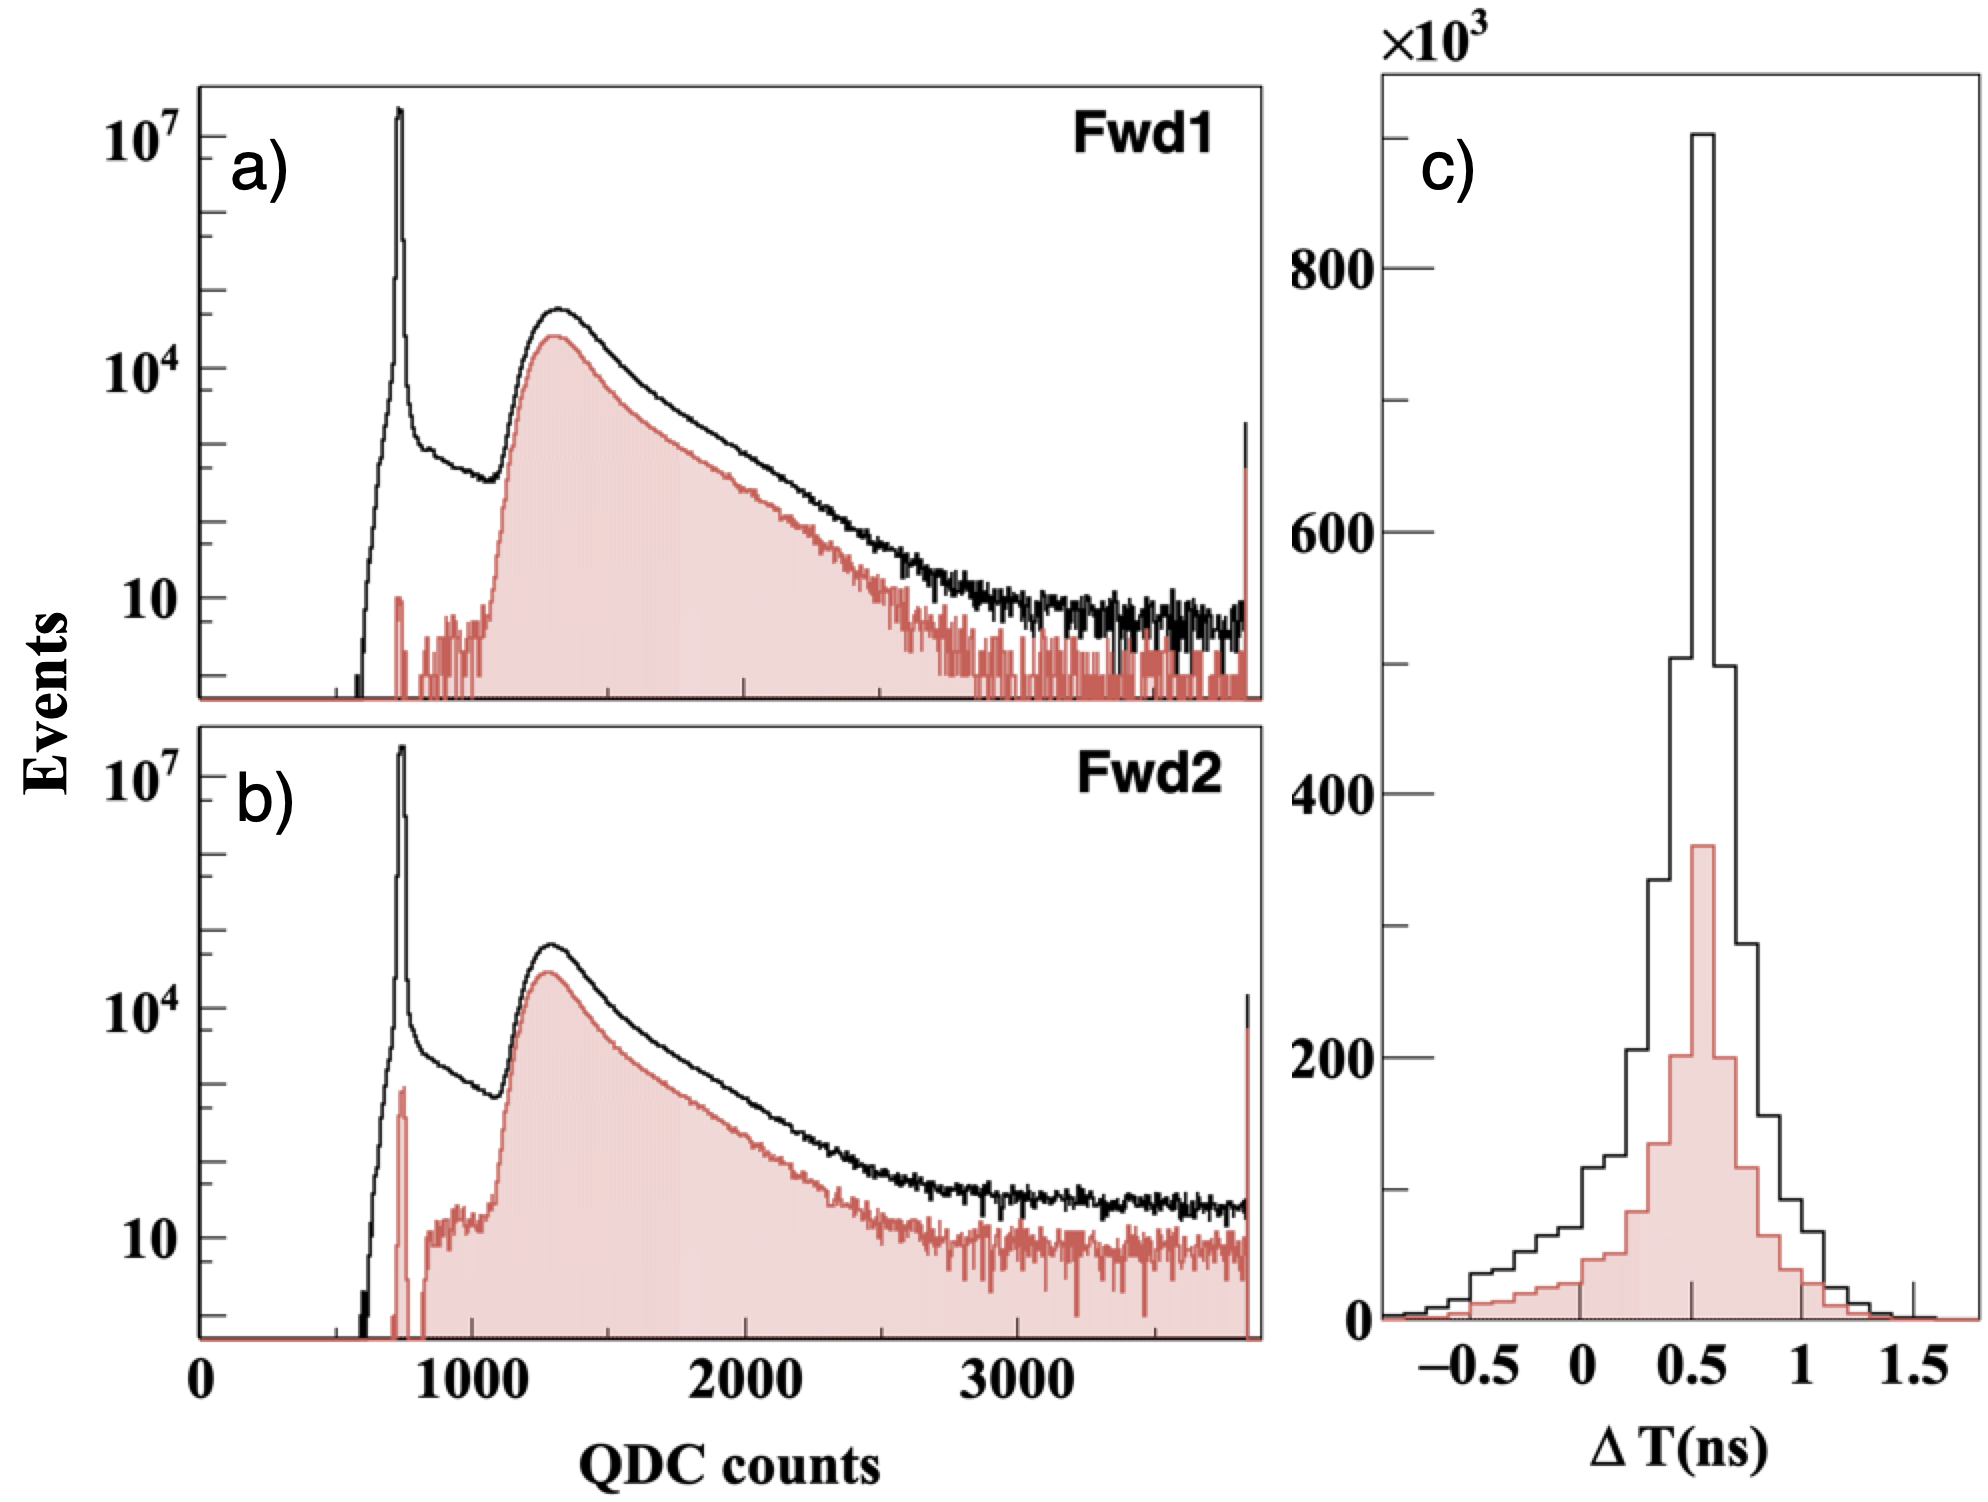
\includegraphics[width=0.48\textwidth]{./fwd_performance_elastic.png}
  \caption{Response of the forward detector: a) the QDC spectrum of the first forward detector module on X arm;
    b) the QDC spectrum of the second forward detector module on X arm; c) Time
    difference distribution between these two modules.
    The black curves are from the events triggered by the recoil
    detector.
    The red shaded curves are from the elastic scattering event sample.
  }
  \label{fig:fwd_performance}
\end{figure}

% A further study is carried out with the sample of elastic scattering events (the selection of the elastic scattering events are described in Sec. \ref{sec:elastic_extraction}).
% The peaks lie above a continuum background, in which no distinctive thresholds can be recognized to separate the noise pedestal and the peak.
A further study is carried out using the tag-and-probe method with a controlled
sample of elastic scattering events.
The response of one module is probed by using the other module to tag the sample
(the procedures for selecting the elastic scattering events are described in Sec. \ref{sec:tofe_selection}).
The results are shown as the red shaded curves in Fig. \ref{fig:fwd_performance}.
The lower limit of the elastic peaks is clearly seen at around \num{1000}.
In the following analysis, this value is used as the threshold for the forward detector.
The corresponding SNRs are about \num{40} for both detector modules.

The detection efficiencies of the forward modules are also determined with the
tag-and-probe method, which are about \SI{99.9978}{\percent} and \SI{99.9560}{\percent}, respectively.
Scattering effects in the first layer reduce the detection efficiency slightly in the second layer.
% Due to the high efficiency, the joint firing of them are required to select a
% valid hit in the forward detector and the hit time is the average of two modules.
The coincidence of both modules is required to have a valid hit in the
forward detector and the hit time is the average of the two modules.

% \subsection{Extraction of elastic scattering peak at large recoil angle}
\subsection{Performance of the recoil detector}
\label{sec:recoil_performance}
The reconstructed energy spectra of the recoil detector show a clear pattern
of elastic scattering in the distribution of the deposited energy versus the
position along the beam axis as shown in Fig. \ref{fig:e_map}.
\begin{figure}[b!]
  \centering
  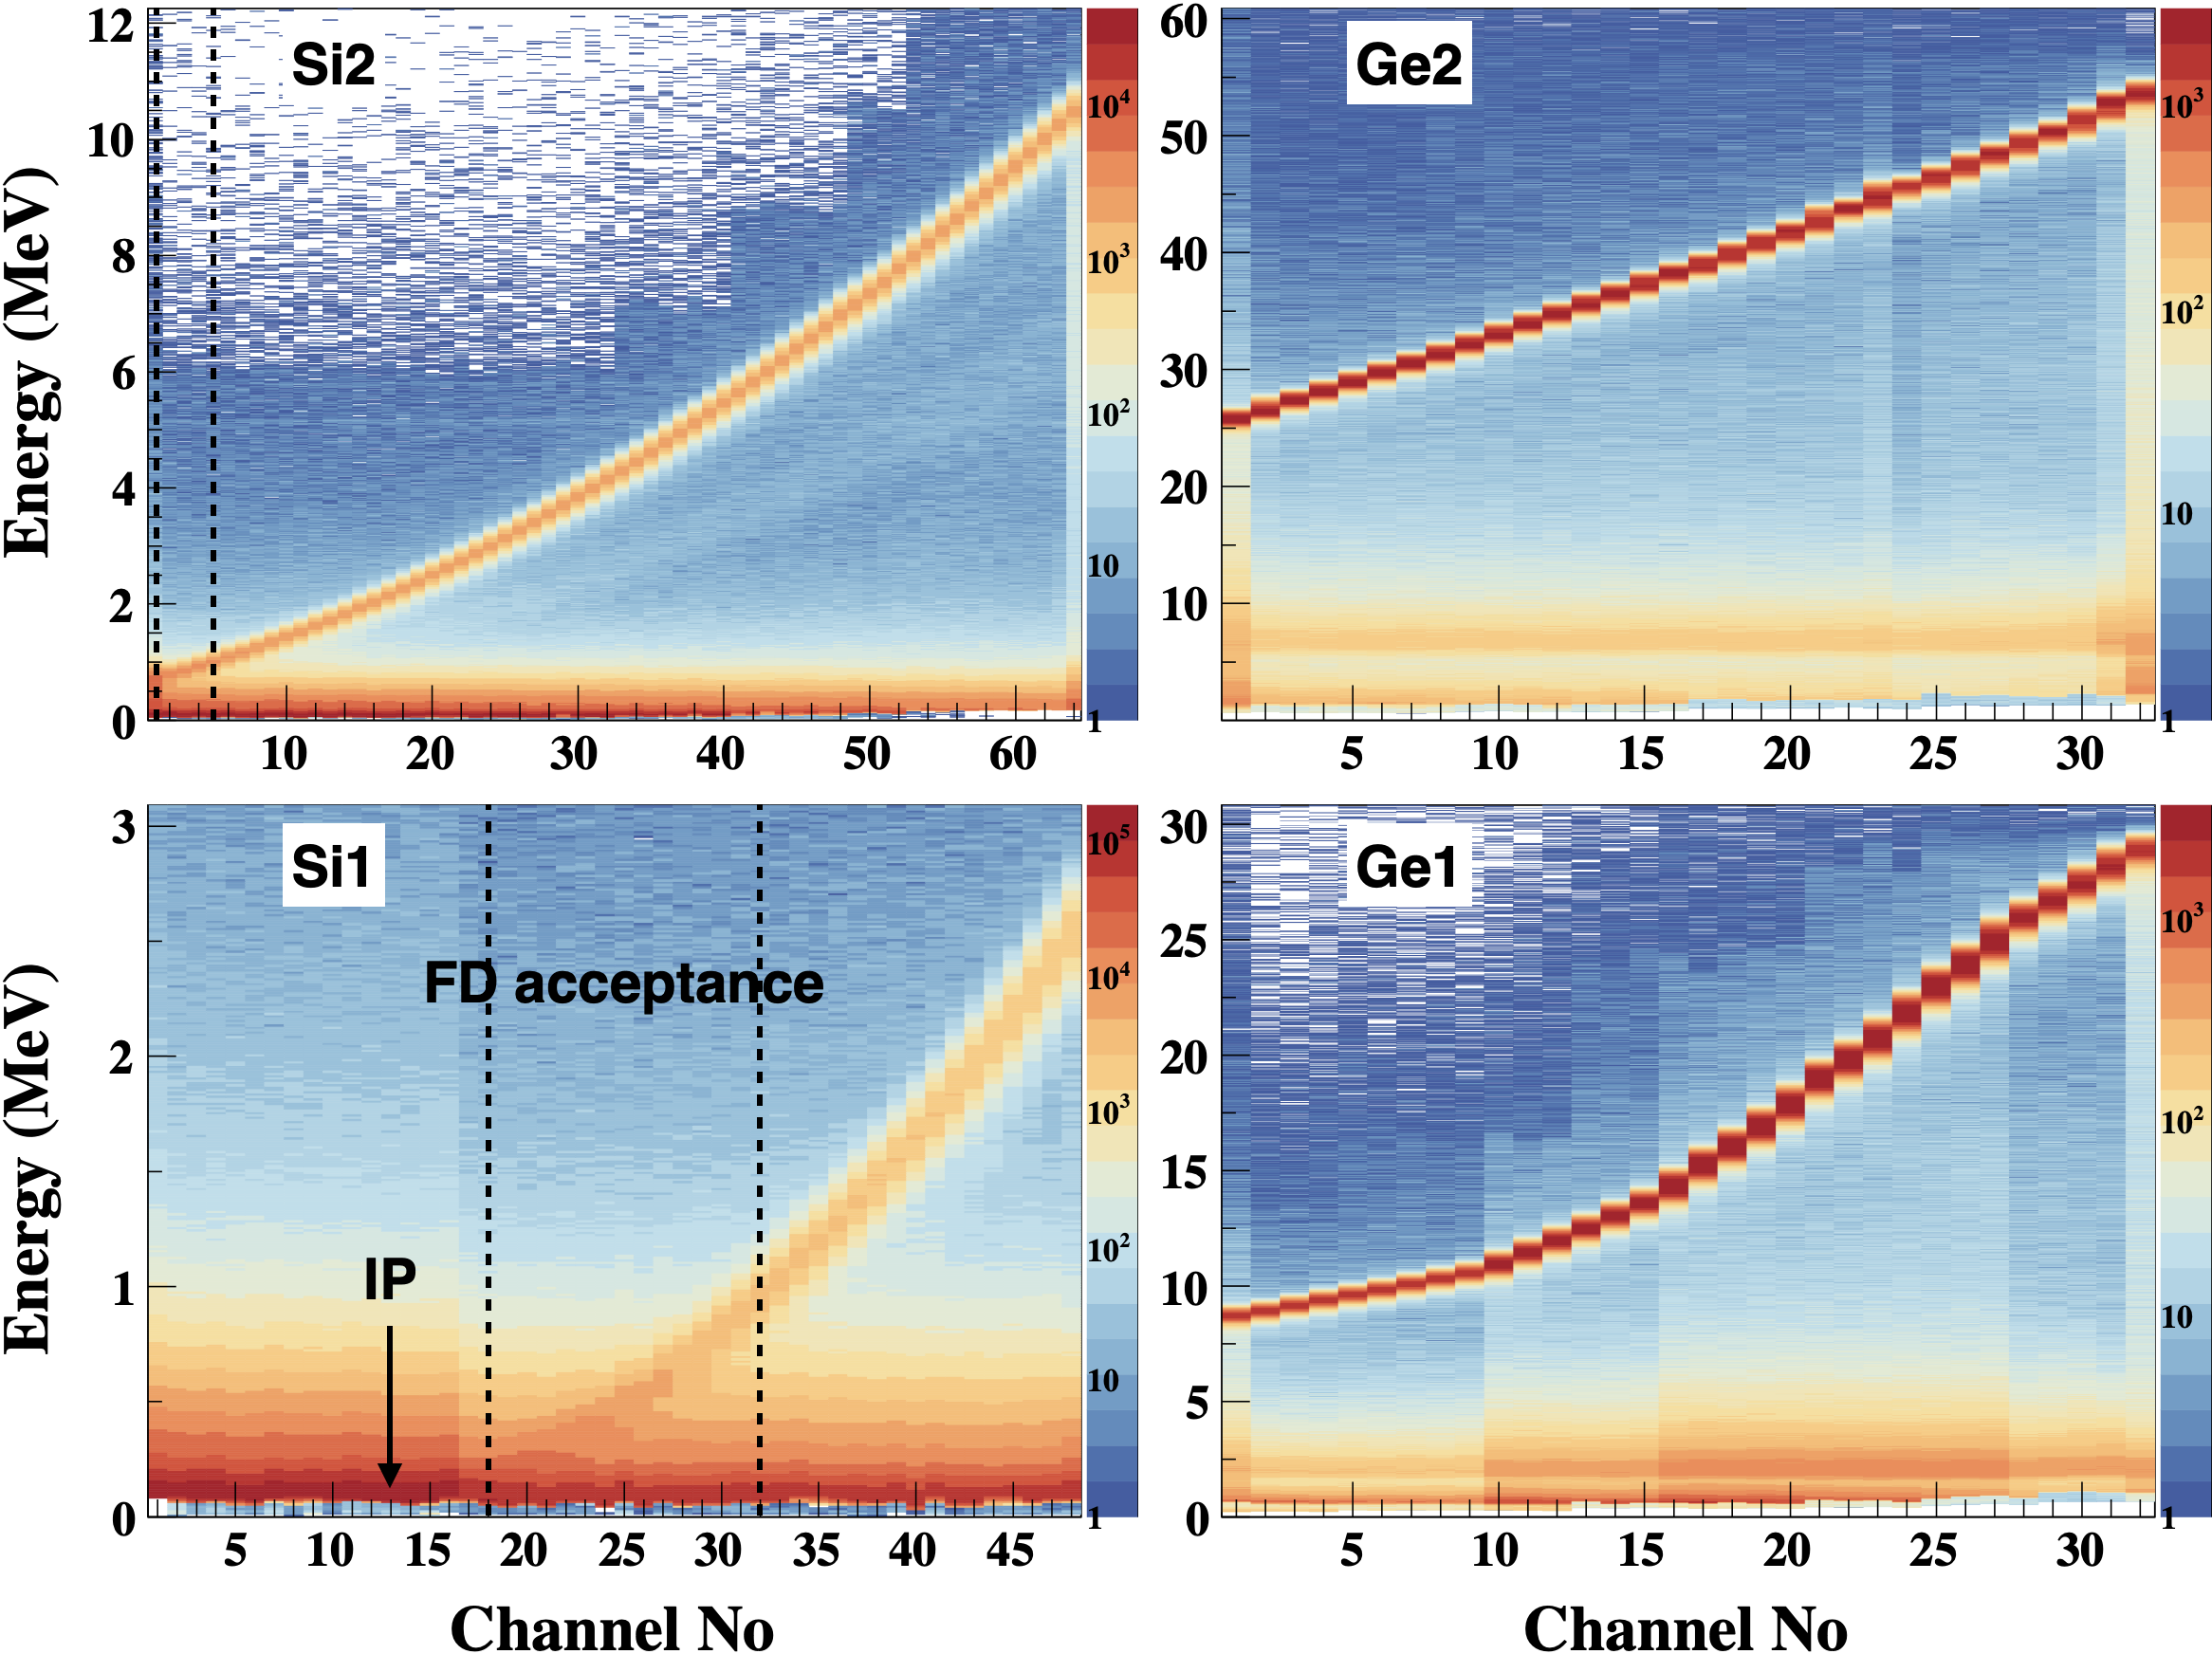
\includegraphics[width=0.48\textwidth]{./e_map.png}
  \caption{Energy spectra (after clustering) for all channels of the four recoil sensors obtained at \SI{2.2}{\momentum}.
    Smaller channel numbers indicate smaller recoil angle.
    IP indicates the channel which is aligned with
    the beam-target center.
    The group of channels which are expected to be fully covered by the forward detector are
    also indicated by the dashed lines on Si1 and Si2.
  }
  \label{fig:e_map}
\end{figure}
The elastic peak is on a wide background, which exists over the whole energy range.
Although the elastic peak is well separated from the low-energy background at
large recoil angles, it becomes hard to distinguish at small recoil angles.
The background consists of three main components:
1) a fast-decreasing exponential component, which has very high yield at low energy;
2) a slow-decreasing exponential component, which extends to high energy;
3) a MIP component, which can be described by a Landau distribution and has a most probable energy deposit of \SI{0.37}{\MeV} in Si1 and Si2, \SI{2.2}{\MeV} in Ge1 and \SI{7.0}{\MeV} in Ge2.
The MIP events are mainly generated by charged pions produced by inelastic events.

The response of each strip to the elastic scattering events from the IP is described
very well by the Crystal-Ball function\cite{crystal_ball}, which is composed of a Gaussian core and a power-law tail on each side of the core.
For the strips at large recoil angle, an accurate estimate of the parameters of
the background components is possible by fitting the sidebands around the elastic peak.
An extended binned Maximum-Likelihood fit over the full energy range above the
trigger threshold, including both the background and the
elastic peak, is then carried out to extract the parameters of the response function and the event rate under the peak.
An example of the combined fit is shown in Fig. \ref{fig:e_fit}.
The sum of multiple Crystal-Ball functions, which share the same shape parameters and
different Gaussian peaks, are used to describe the response of the readout channel with multi-strips. 
% The standard one-sided Crystal-Ball distribution is expanded to double sides, which is composed of a Gaussian core and two
% power-law tails at low-end and high-end of the core.
% The extracted width of the response function core varies with the peak energy and the
% equivalent Fano factor is about 185 larger than the one obtained using $\alpha$
% source, which is about 17 in terms of FWHM.
The intrinsic resolution of the recoil sensor determined from the $\alpha$ source
calibration ($\sim$\SI{20}{\keV} FWHM at \SI{5}{\MeV}) is much smaller than the
extracted width of the elastic peak from the beam data ($\sim$\SI{330}{\keV}
FWHM at \SI{5}{\MeV}).
Thus, the width of the energy peak is mainly dominated by the finite
angular coverage of the strip and the thickness of the cluster jet target along the beam direction.
\begin{figure}[tb!]
  \centering
  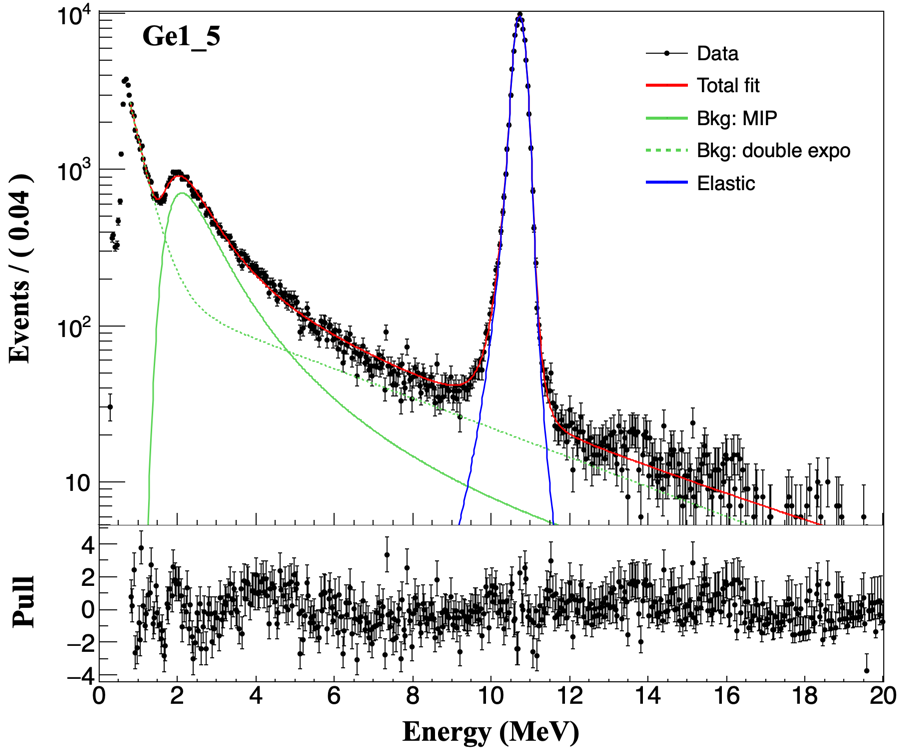
\includegraphics[width=0.45\textwidth]{./e_fit.png}
  \caption{Extraction of the elastic peak spectrum using the extended binned
    Maximum-Likelihood fit. Three components are used in the background model
    and the fit is carried out over the full range indicated. The pull of each bin
    is shown in the bottom frame.}
  \label{fig:e_fit}
\end{figure}

The accuracy of the combined fit deteriorates at small recoil angles, where the elastic peak approaches the MIP peak and both peaks are embedded among the large
low-energy background ($\lesssim$ \SI{1}{\MeV}).
In this case, the fit parameters become strongly correlated and there is a large error in determining the fraction of each component.
A pre-selection of the elastic scattering events is needed to get a cleaner spectrum.
For the strips which are covered by the forward detector, the coincidence between the recoil proton and the scattering beam particle is utilized for this selection.

% The fitting model is composed as follows,
% \begin{equation}
% \begin{aligned}
% \mathcal{P}(x) &= N_{1}\lambda_1e^{-\lambda_{1}x}+N_{2}\lambda_2e^{-\lambda_{2}x}\\
% &+N_{3}\mathcal{L}(x;\mu_{mip},\sigma_{mip})\ast\mathcal{N}(x;\sigma_{gaus})\\
% &+N_{4}\sum_{i=1}^{n_{strips}}{c_{i}f(x;\mu_{i},\sigma_{cb},\alpha_1,n_1,\alpha_2,n_2)}
% \mathcal{P}(x) &= N_{1} \cdot exp(x;\lambda_{1}) + N_{2} \cdot exp(x;\lambda_{2})\\
% &+ N_{3}\cdot L(x;\mu_{mip},\sigma_{mip}, \sigma_{res})\\
% &+ N_{4}\cdot \sum_{i=1}^{n_{strips}}{c_{i}f_{cb}(x;\mu_{i},\sigma_{cb},\alpha_1,n_1,\alpha_2,n_2)}
% \end{aligned}
% \end{equation}
% where the first two items are the exponential components, the third item is the
% normalized landau distribution convoluted with the Gaussian response function
% and the fourth item is the response function of the recoil detector to the
% elastic scattering events from the target.
% $N_i (i=1,2,3,4)$ is the event counts for each component of the model.
% The double-sided crystal ball function is composed of a Gaussian core and two
% power-law tails as follows,
% \begin{multline}
%   f(x;\mu,\sigma,\alpha_1,n_1,\alpha_2,n_2) = \\
%   N\cdot
%   \begin{cases}
%     \exp(-\frac{(x-\mu)^2}{2\sigma^2}), &\text{for } \alpha_1 < \frac{(x-\mu)}{\sigma} < \alpha_2\\
%     A_1(B_1-\frac{x-\mu}{\sigma})^{-n_1}, &\text{for } \frac{(x-\mu)}{\sigma} \leqslant \alpha_1\\
% 	    A_2(B_2+\frac{x-\mu}{\sigma})^{-n_2}, &\text{for } \frac{(x-\mu)}{\sigma} \geqslant \alpha_2
%   \end{cases} 
% \end{multline}
% where
% \begin{align}
%   A_i &= (\frac{n_i}{\abs{\alpha_i}})^{n_i}\cdot\exp(-\frac{\alpha_i^2}{2}) &,(i=1,2)\\
%   B_i &= \frac{n_i}{\abs{\alpha_i}} - \abs{\alpha_i} &,(i=1,2)
% \end{align}

\subsection{Event selection with the TOF-E relation}
\label{sec:tofe_selection}

Most background events are already suppressed by requiring the forward detector to have a valid hit from the beam particle.
A more accurate selection of elastic scattering events is achieved by using the TOF-E relation.
The time-of-flight of the recoil proton and its kinetic energy (E)
have a fixed relation $TOF = l\sqrt{m_p/2E}$, where $l$ is the distance of
the recoil detector to the IP and $m_p$ is the proton mass.
Due to the negligibly small variation of the flight time of the scattering beam particle,
the TOF of the recoil proton can be approximated by the difference between the hit time of the recoil detector and the forward detector.

% Elastic selection based on TOF-E
% The typical TOF-E spectrum from a single strip is shown in the inner subplot of Fig. \ref{fig:tof-e}.
Two bands of events connect to the elastic peak and are observed in the raw TOF-E spectrum for each strip, as shown in the inset of Fig. \ref{fig:tof-e}.
Both bands are generated by the recoil protons of elastic scattering, with:
\begin{enumerate*}[label=(\roman*)]
\item band A from the interaction of the beam particle with the residual gas in the scattering chamber;
\item band B from the events in which the recoil protons hit the edge of the strip and only deposit part of their energy in the sensor.
\end{enumerate*}
\begin{figure}[b!]
  \centering
  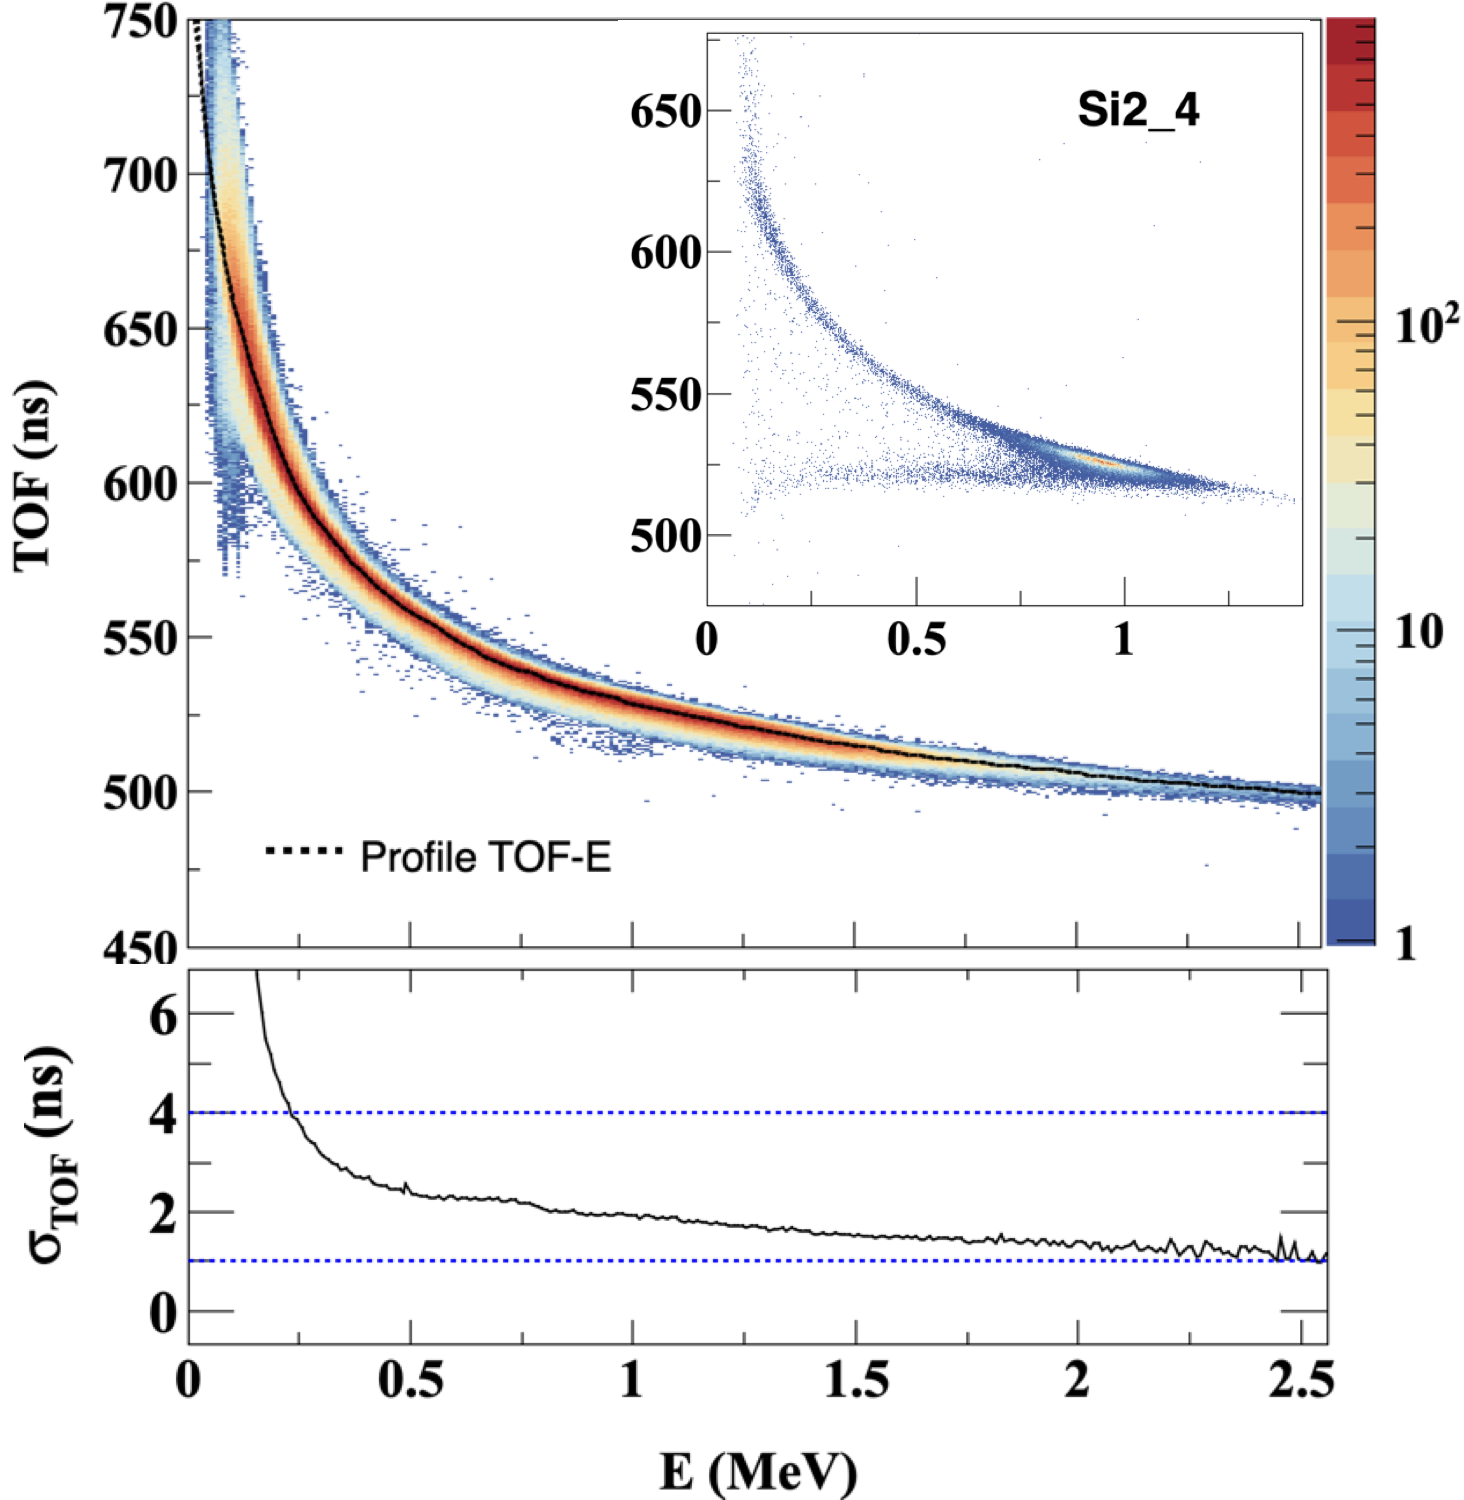
\includegraphics[width=0.42\textwidth]{./tofe_tsigma.png}
  % 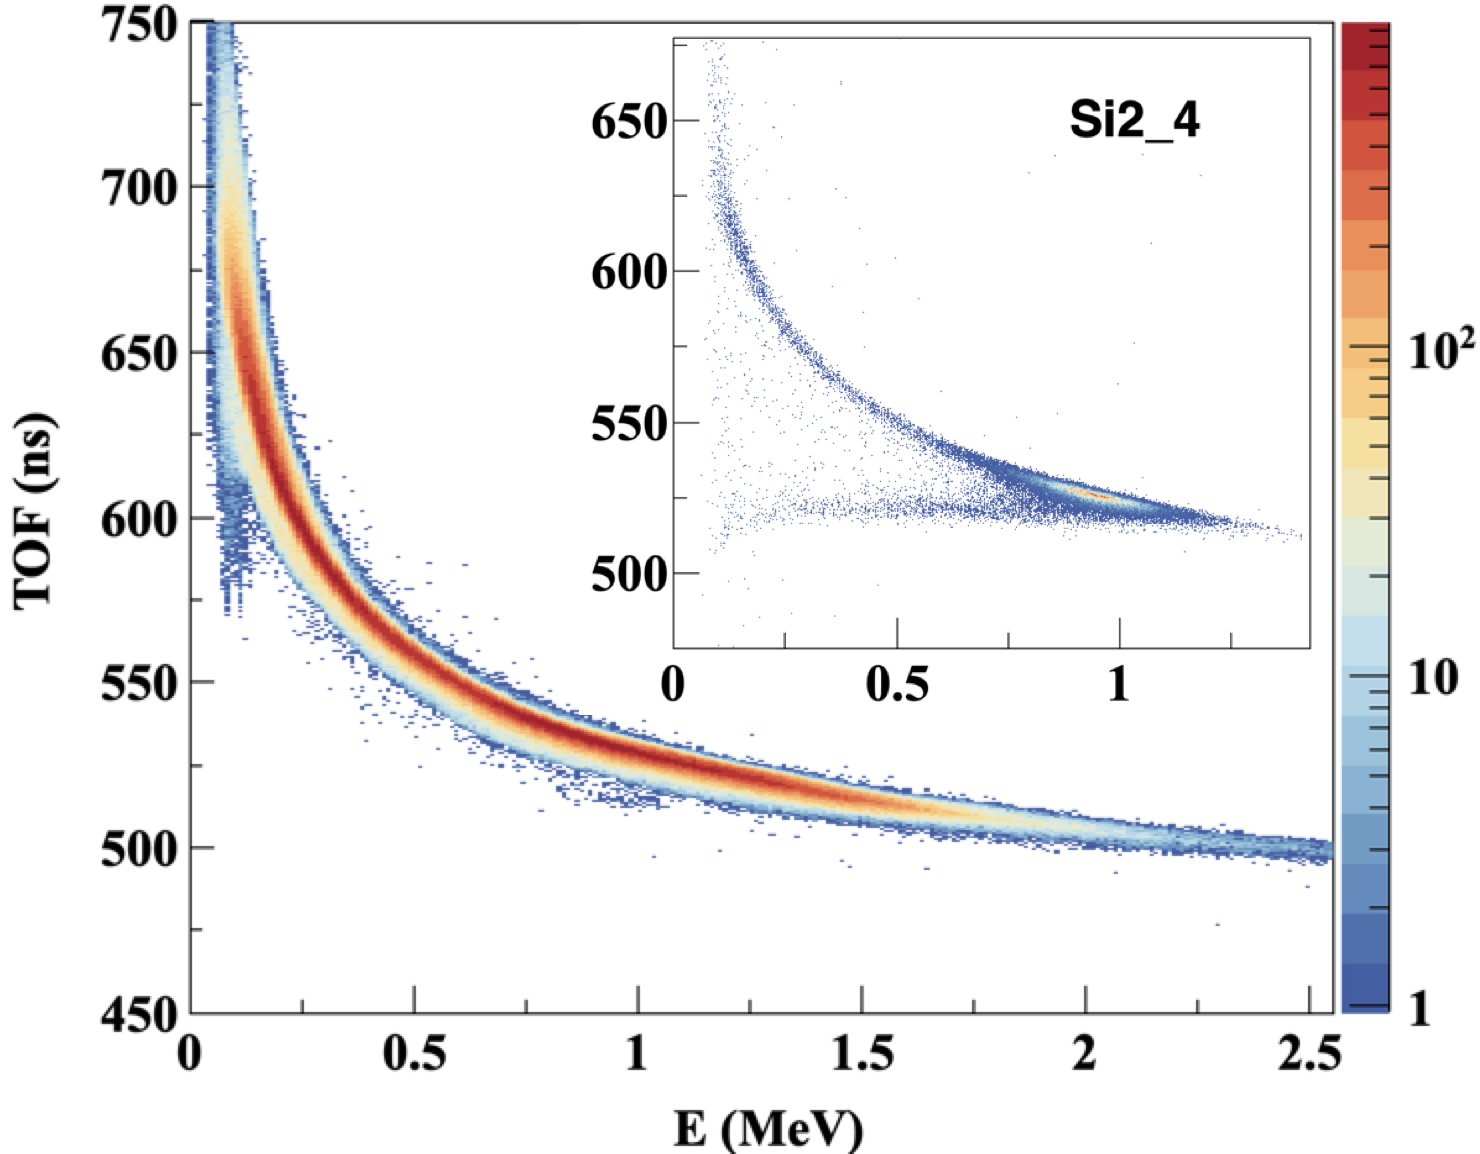
\includegraphics[width=0.4\textwidth]{./tofe_cut.png}
  \caption{
    The upper frame shows the TOF-E spectrum of all strips for selected elastic
    scattering events at \SI{2.2}{\momentum}.
    A typical raw TOF-E spectrum for a single strip is shown in the inset, here region C is the elastic peak.
    The lower frame shows the time resolution for $\SI{10}{\keV}$ bins of energy.
    }
  \label{fig:tof-e}
\end{figure}
The events of the elastic peak (region C in Fig. \ref{fig:tof-e}) and band A are selected roughly and filled into an overall TOF-E spectrum of elastic scattering events from all strips.
This spectrum is divided into \SI{10}{\keV} steps,  and a smooth, data-deduced TOF-E curve is obtained as shown in the main plot of Fig. \ref{fig:tof-e}.
The standard deviation of TOF ($\sigma_{TOF}$) for each step is also extracted and shown in the bottom frame of Fig. \ref{fig:tof-e}.
$\sigma_{TOF}$ reaches an asymptotic value of $\sim$\SI{1}{\ns} for high energies, which can be considered as the intrinsic timing resolution of the recoil
detector since the forward detector has much better resolution (see Sec. \ref{sec:fwd_performance}).
At $E < \SI{250}{\keV}$, $\sigma_{TOF}$ deteriorates rapidly because of the
combined effect of the finite energy resolution and the large derivative of the TOF-E relation.
% This selection effectively filter out all the full elastic events as show in the
% main plot of Fig. \ref{fig:tof-e}.
% \textit{i.e.} elastic events in which the recoil proton deposit all its energy in the recoil sensor and the scattered proton penetrating through the forward detector. 
% The TOF-E spectrum The selected events from all of this selection is shown in Fig. \ref{fig:tof-e}.
% with the two side plots showing the variation of the
% standard deviation ($\sigma_{TOF}$ and $\sigma_{E}$) of the profile along the E-axis and TOF-axis respectively.
% The deteoriation of the resolution near the edge of the spectrum is mainly
% contributed by the extremely large or small derivative of the TOF-E curve at
% these energy values.
% The modest value of $\sigma_{TOF}$ and $\sigma_{E}$ is about
% \SI{2.5}{\nano\second} and \SI{25}{\keV} respectively.

% combined fit using coulomb background and coverage of the fwd acceptance
% The TOF-E curve is combined with a $[-5\sigma_{TOF}, 5\sigma_{TOF}]$ window to select the elastic scattering events on each strip.
Events within $\pm 5\sigma_{TOF}$ of the TOF-E curve are selected as the elastic
scattering events.
A clean energy spectrum is obtained after the selection and the elastic peak shows up clearly.
The results for three strips at different recoil angles are shown in Fig. \ref{fig:cut}.
\begin{figure}[b!]
  \centering
  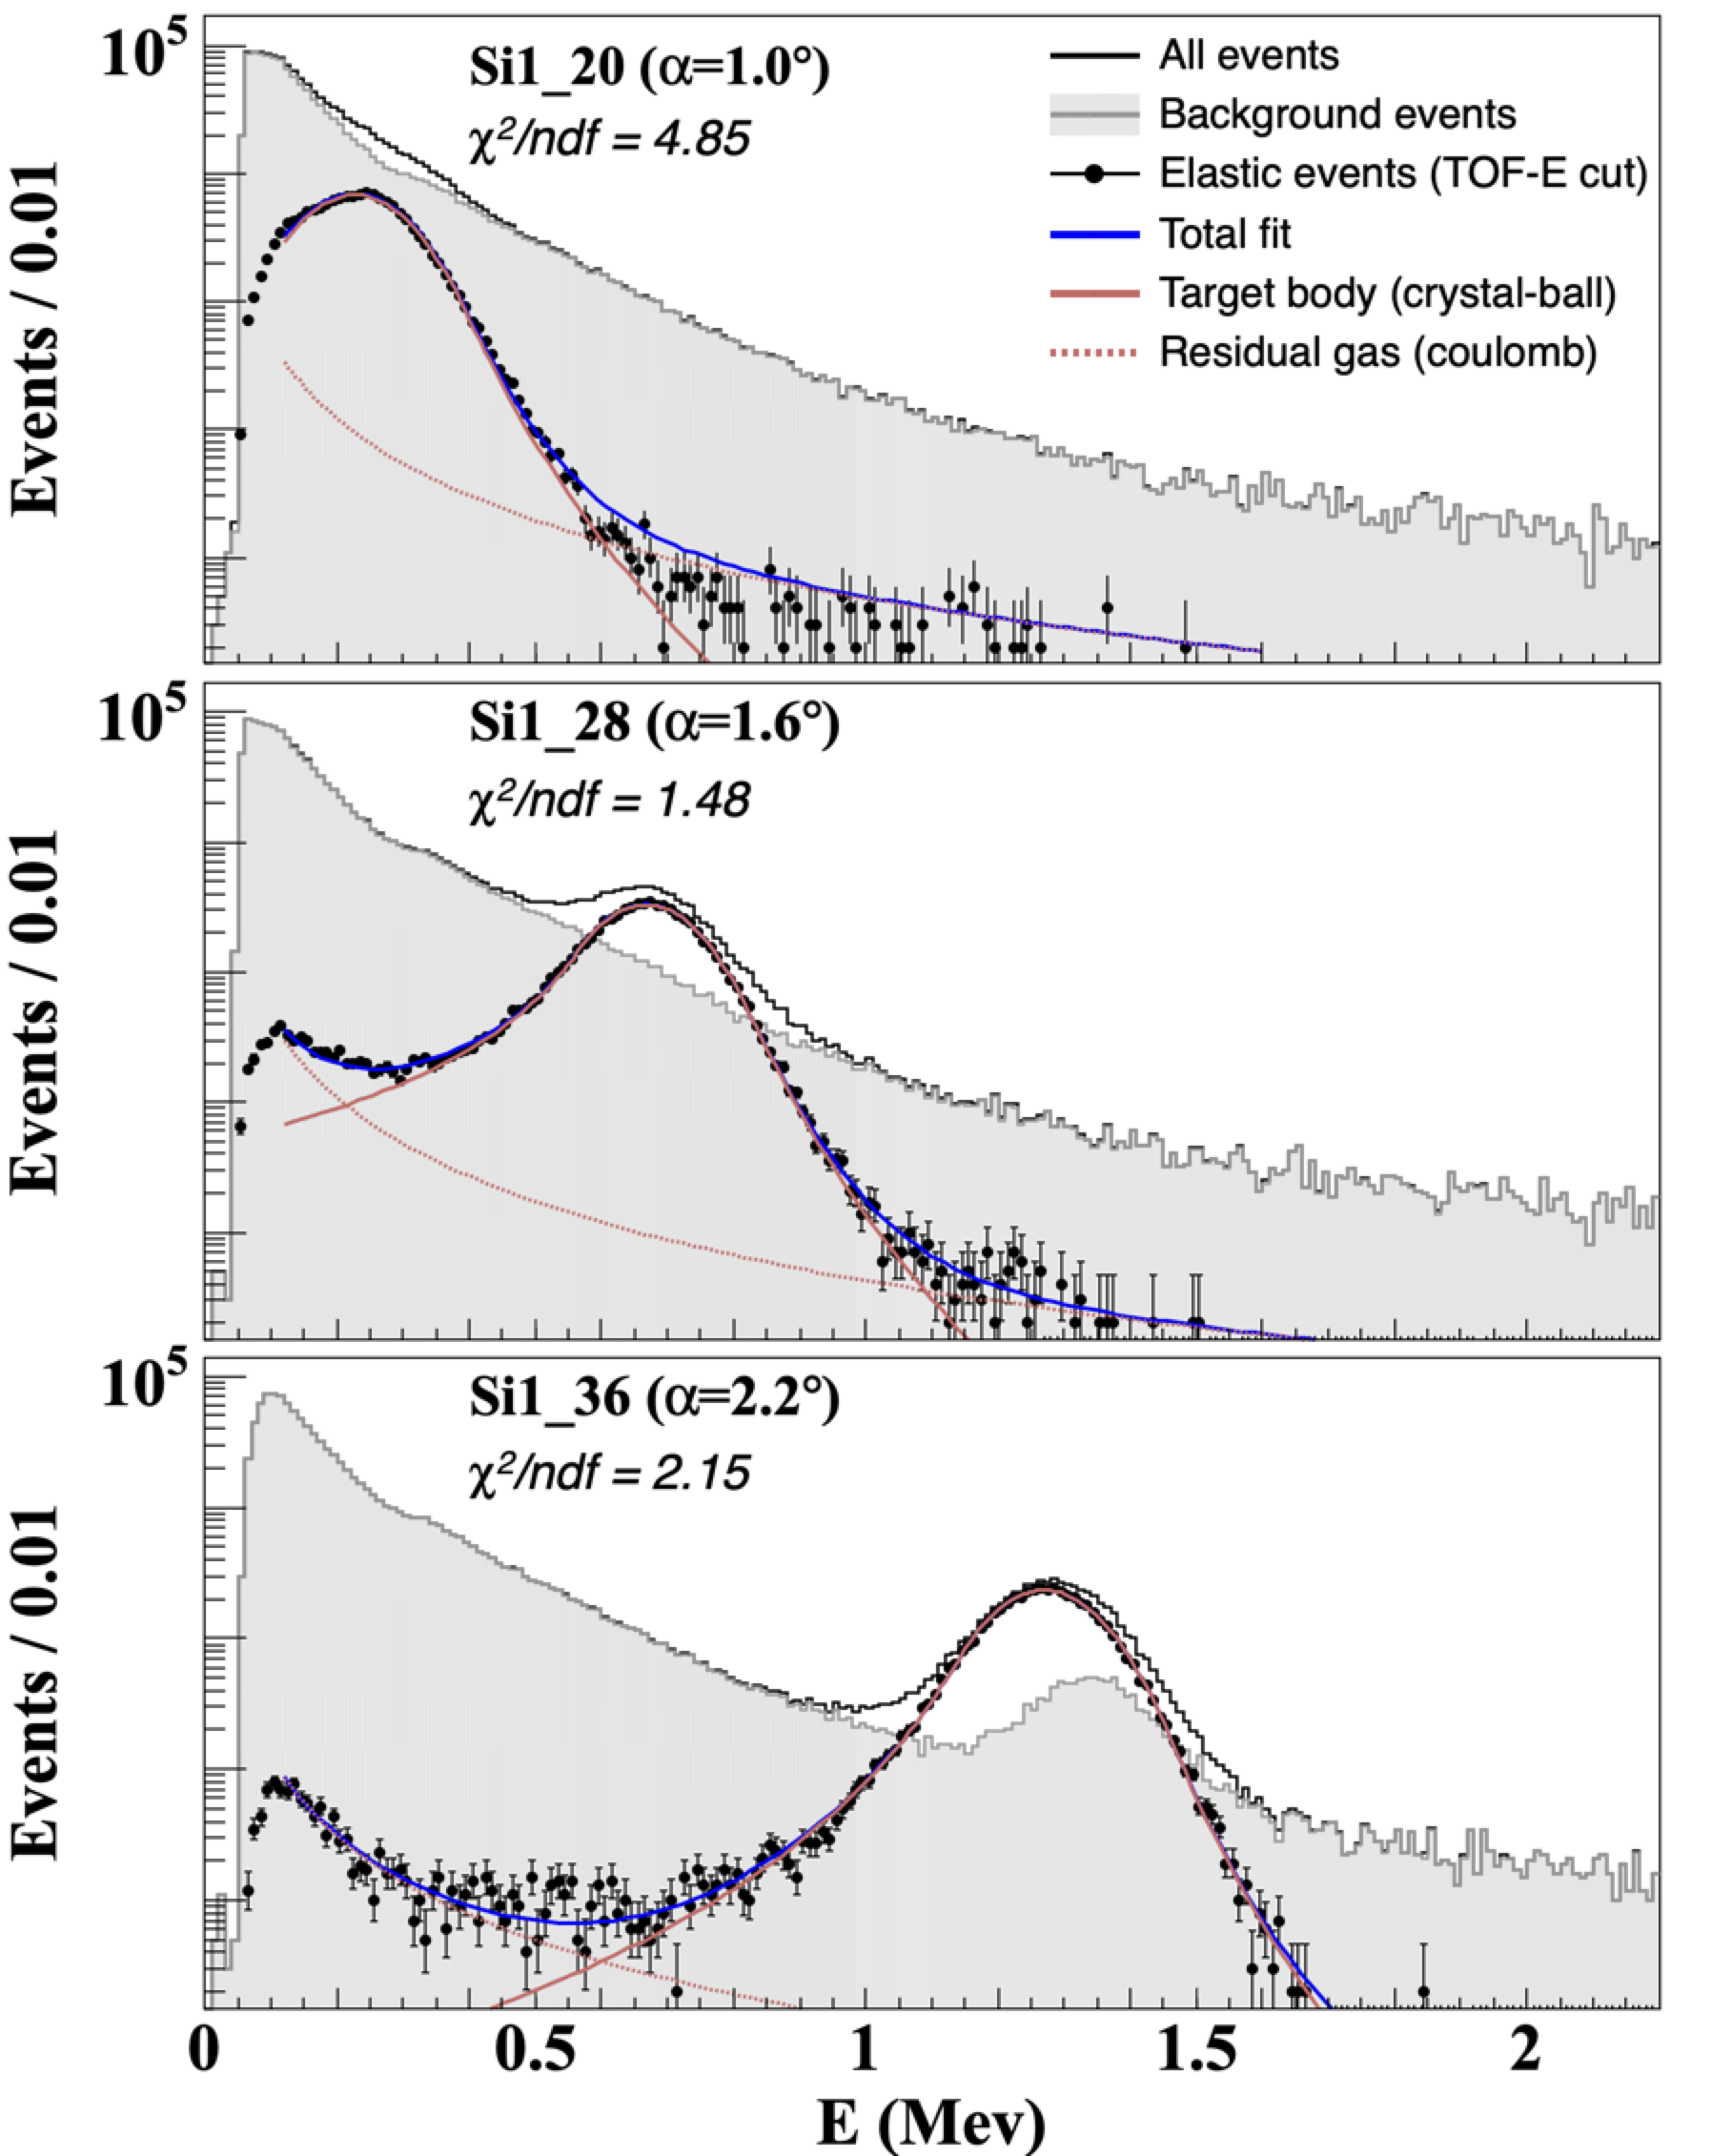
\includegraphics[width=0.45\textwidth]{./tofe_cut_comparison.png}
  \caption{The energy spectra of TOF-E selected events (black dots) from strips
    at three recoil angles. The black lines are the spectra from all events and
    the grey spectra are rejected events that have no coincidence with the forward detector.}
  \label{fig:cut}
\end{figure}
For strips which are fully covered by the forward detector, the spectrum of the
suppressed background events has a smooth transition over the elastic peak range
as shown in Fig. \ref{fig:cut} (b).
This indicates a high efficiency of the selection condition.
With increasing recoil angle, the forward detector gradually loses the full coverage
of the recoil strip and a small elastic peak appears in the background spectrum
as shown in Fig. \ref{fig:cut} (c).
On the other hand, with decreasing recoil angle, the finite thickness of the
cluster jet target can not be ignored and the forward detector starts to lose the coverage of the full target profile due
to the lower limit of the acceptance as shown in Fig. \ref{fig:cut} (a).
In comparison to Fig. \ref{fig:forward_acceptance}, the strips with all events
inside the red box are shown here in Fig. \ref{fig:cut} (b).
The strips where some of the events are lost above or below the red box are
shown in Fig. \ref{fig:cut} (c).
Strips with a significant fraction of events located near the vertical red line
at $X = \SI{3}{\cm}$ are shown in Fig. \ref{fig:cut} (a).

The remaining background in the selected events comes from elastic scattering
off the residual gas, which is mainly the hydrogen atoms from the evaporation
off the cluster jet beam \cite{cluster_target}.
The shape of this background is well described by the Coulomb elastic scattering cross
section, due to the uniform distribution of the residual gas and the rapid decrease of the elastic scattering cross section beyond the Coulomb region.
Again, an extended unbinned Maximum-Likelihood fit with a sum of the Coulomb elastic scattering formula and the Crystal-Ball
function is used to extract the parameters of the response function and the
yield of elastic events from the core of the cluster jet stream. 
Fit results for the three example strips are also shown in Fig. \ref{fig:cut}.
It's found that the fit quality deteriorates when the full shape of the target profile is not available.
This limits the lower range of the $|t|$ measurement to $\sim$\SI{0.001}{\tmom} at $P_{beam}=\SI{2.2}{\momentum}$.

\subsection{Minimum measurable $|t|$}
\label{sec:minimum_t}
\begin{figure}[b!]
  \centering
  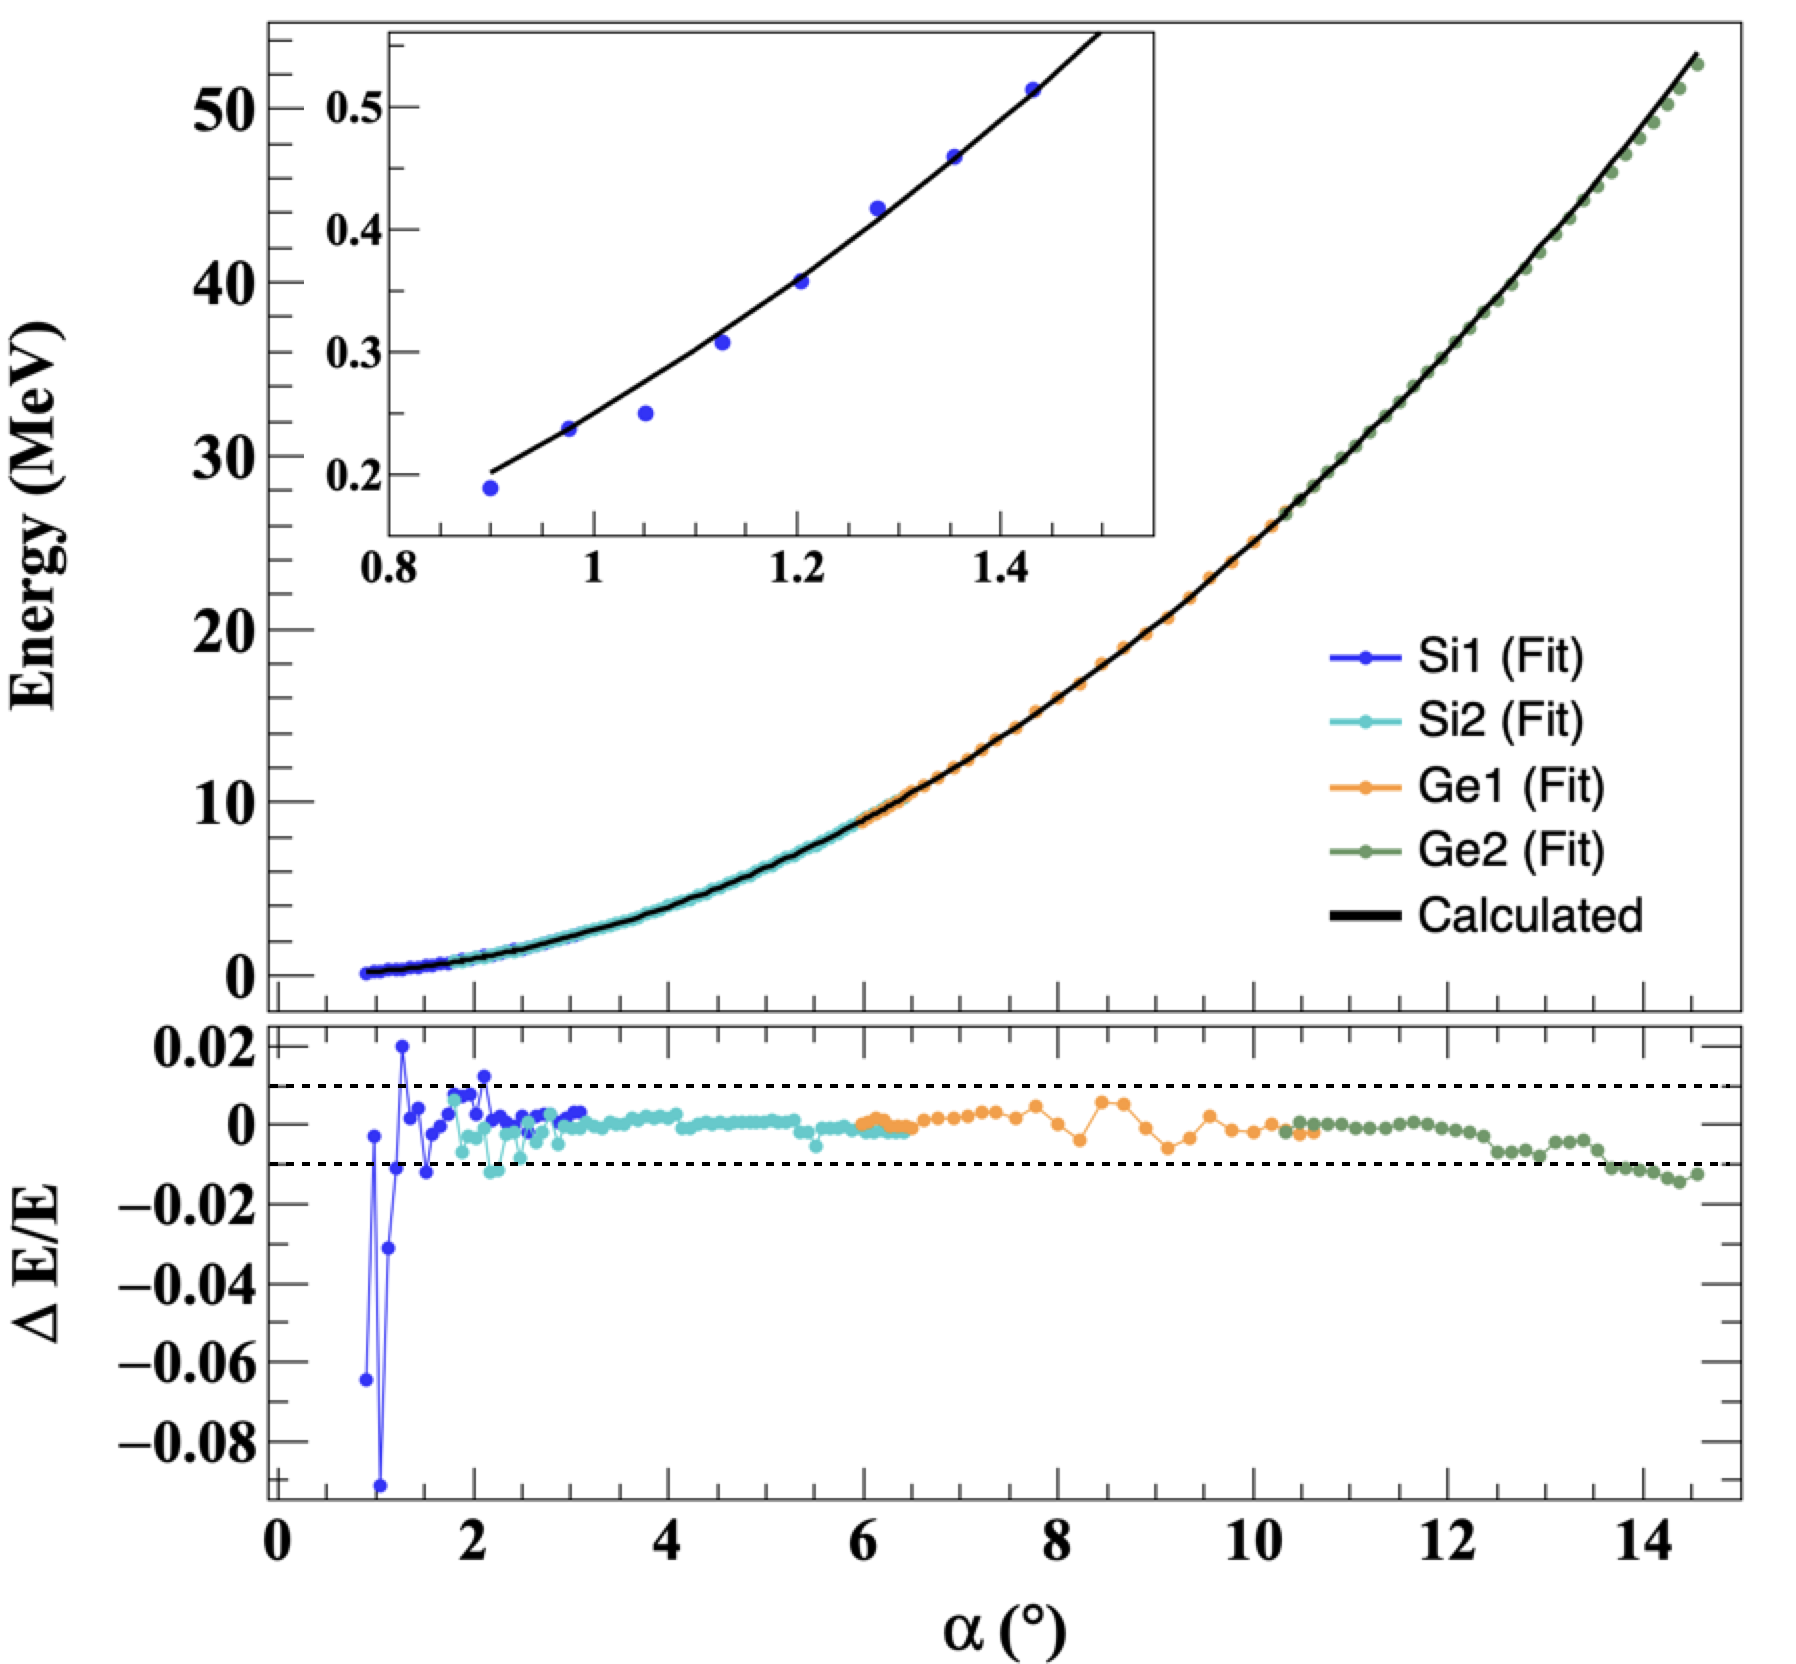
\includegraphics[width=0.45\textwidth]{./e_vs_alpha_combined.png}
  \caption{
    Comparison of the measured (colored dots) and the calculated (black line)
    recoil energy on the strip center at different recoil angles. The relative
    difference is drawn in the bottom plot. The results are for $P_{beam} = \SI{2.2}{\momentum}$.}
  \label{fig:measured_vs_calculated}
\end{figure}
The spectra of the suppressed background events on the strips, which are fully covered by the
forward detector, can be used as the template model to describe the background
shape for strips at smaller recoil angles.
Thus, the lower range of the $|t|$ measurement can be extended below the limit set by the TOF-E selection method.
The scaling parameter of the background model is first estimated with the upper
sideband of the energy spectrum, and a combined fit with the sum of the Crystal-Ball function and the background template is then carried
out over the full energy range to extract the elastic peak spectrum.

% A limit is observed around \SI{350}{\keV}, which corresponds to $|t| \approx  \SI{0.0007}{\tmom}$.
The limit of the method is reflected in the extracted elastic peak energy on each strip as shown in
Fig. \ref{fig:measured_vs_calculated}.
For the strips where the full elastic peak spectrum is extracted and described accurately
by the Crystal-Ball function, the relative difference between the measured and
the calculated recoil energy based on kinematic relations is within \SI{\pm 1}{\percent}.
The discrepancy enlarges rapidly at $\alpha < \SI{1.2}{\degree}$ when part of
the target profile is not recorded by the recoil strips due to the trigger threshold.
Both the extracted parameters of the response function and the event rate have large uncertainties in this case.
The observed lower limit of the energy peaks is about \SI{350}{\keV} at \SI{2.2}{\momentum}, which corresponds to the minimum measurable $|t|$ of $\sim$\SI{0.0007}{\tmom}.

\section{Conclusion and outlook}
\label{sec:conclusion}

The commissioning of the full KOALA setup at COSY, specifically of the new forward detector, was successful.
A strong correlation between the recoil detector and the forward detector is
observed for the kinematic region covered by the forward detector.
The discriminating power of using the TOF-E relation of the recoil proton to select elastic
scattering events is verified.
Preliminary analysis shows that the lower |t| range can be extended slightly beyond the design goal of \SI{0.0008}{\tmom}.

The finite thickness of the target profile can not be ignored at
very small recoil angles ($\alpha < \SI{1.2}{\degree}$) and it greatly
constrains the lower limit of the $|t|$ measurement.
% The integral thickness of the target profile along the beam-axis is estimated to
% be $\sim$\SI{5.6}{\mm} (FWHM), which is much larger than the design value.
The observed integral thickness of the target profile is larger than the design value.
Since the stochastic cooling was not stable during the beam commissioning, this may be caused by the combined effect of the tilting of the cluster jet
beam and the unexpected large emittance of the COSY beam.
An investigation of the cluster target setup is ongoing and more stable stochastic cooling is required in the future experiments.
Furthermore, a larger size of the forward scintillators, especially a larger width, is also proposed.

The DAQ was operated in a stable condition during the beam commissioning.
It was noted that the trigger bias could occur if the high noisy signal channels of the sensors were involved into the trigger
logic. In order to avoid the potential trigger bias, those signal
channels should be removed from the trigger logic for the future
measurements.

% % The event synchronization based on the mask gate was used.
% However, bias of the trigger efficiency is observed among different
% sensors of the recoil detector by checking the elastic event counts on overlapping strips.
% This is caused by the different electronic noise level on each recoil sensor and
% the limited performance of the mask gate based event synchronization at high
% rate triggers.
% Due to the self-triggering design, noise triggering levels will change
% the corresponding trigger efficiency once the DAQ efficiency limit is reached.
% It was also found that only several strips before the interaction point
% contribute to the high rate noisy triggers.
% Thus, these noisy strips are proposed to be removed from the trigger logic in the future experiment.

These results show that the KOALA setup is ready to be used at HESR, with modifications only needed
to renew specific haredware components of the target setup and to assemble a new
beam pipe between the target chamber and the forward detector. 

\section{Acknowledgement}
\label{sec:acknowledgement}
We are grateful to the COSY crew for providing proton beams for tests.
We are indebted to the COSY vacuum team who managed to install the KOALA
setup into the COSY ring. Special thanks are dedicated to Tamas
Vashegyi, who implemented the beam timing receiver for the trigger logic.

\bibliographystyle{elsarticle-num}
\bibliography{reference}

\end{document}
